% This is "sig-alternate.tex" V2.1 April 2013
% This file should be compiled with V2.5 of "sig-alternate.cls" May 2012
%
% This example file demonstrates the use of the 'sig-alternate.cls'
% V2.5 LaTeX2e document class file. It is for those submitting
% articles to ACM Conference Proceedings WHO DO NOT WISH TO
% STRICTLY ADHERE TO THE SIGS (PUBS-BOARD-ENDORSED) STYLE.
% The 'sig-alternate.cls' file will produce a similar-looking,
% albeit, 'tighter' paper resulting in, invariably, fewer pages.
%
% ----------------------------------------------------------------------------------------------------------------
% This .tex file (and associated .cls V2.5) produces:
%       1) The Permission Statement
%       2) The Conference (location) Info information
%       3) The Copyright Line with ACM data
%       4) NO page numbers
%
% as against the acm_proc_article-sp.cls file which
% DOES NOT produce 1) thru' 3) above.
%
% Using 'sig-alternate.cls' you have control, however, from within
% the source .tex file, over both the CopyrightYear
% (defaulted to 200X) and the ACM Copyright Data
% (defaulted to X-XXXXX-XX-X/XX/XX).
% e.g.
% \CopyrightYear{2007} will cause 2007 to appear in the copyright line.
% \crdata{0-12345-67-8/90/12} will cause 0-12345-67-8/90/12 to appear in the copyright line.
%
% ---------------------------------------------------------------------------------------------------------------
% This .tex source is an example which *does* use
% the .bib file (from which the .bbl file % is produced).
% REMEMBER HOWEVER: After having produced the .bbl file,
% and prior to final submission, you *NEED* to 'insert'
% your .bbl file into your source .tex file so as to provide
% ONE 'self-contained' source file.
%
% ================= IF YOU HAVE QUESTIONS =======================
% Questions regarding the SIGS styles, SIGS policies and
% procedures, Conferences etc. should be sent to
% Adrienne Griscti (griscti@acm.org)
%
% Technical questions _only_ to
% Gerald Murray (murray@hq.acm.org)
% ===============================================================
%
% For tracking purposes - this is V2.0 - May 2012

\documentclass{sig-alternate-05-2015}


\begin{document}

% Copyright
\setcopyright{acmcopyright}
%\setcopyright{acmlicensed}
%\setcopyright{rightsretained}
%\setcopyright{usgov}
%\setcopyright{usgovmixed}
%\setcopyright{cagov}
%\setcopyright{cagovmixed}

%
% --- Author Metadata here ---
%\CopyrightYear{2007} % Allows default copyright year (20XX) to be over-ridden - IF NEED BE.
%\crdata{0-12345-67-8/90/01}  % Allows default copyright data (0-89791-88-6/97/05) to be over-ridden - IF NEED BE.
% --- End of Author Metadata ---

\title{Twitter Bot Behavior: How Twitter Bots Interact With People}
\subtitle{}
%
% You need the command \numberofauthors to handle the 'placement
% and alignment' of the authors beneath the title.
%
% For aesthetic reasons, we recommend 'three authors at a time'
% i.e. three 'name/affiliation blocks' be placed beneath the title.
%
% NOTE: You are NOT restricted in how many 'rows' of
% "name/affiliations" may appear. We just ask that you restrict
% the number of 'columns' to three.
%
% Because of the available 'opening page real-estate'
% we ask you to refrain from putting more than six authors
% (two rows with three columns) beneath the article title.
% More than six makes the first-page appear very cluttered indeed.
%
% Use the \alignauthor commands to handle the names
% and affiliations for an 'aesthetic maximum' of six authors.
% Add names, affiliations, addresses for
% the seventh etc. author(s) as the argument for the
% \additionalauthors command.
% These 'additional authors' will be output/set for you
% without further effort on your part as the last section in
% the body of your article BEFORE References or any Appendices.

\numberofauthors{2} %  in this sample file, there are a *total*
% of EIGHT authors. SIX appear on the 'first-page' (for formatting
% reasons) and the remaining two appear in the \additionalauthors section.
%
\author{
% You can go ahead and credit any number of authors here,
% e.g. one 'row of three' or two rows (consisting of one row of three
% and a second row of one, two or three).
%
% The command \alignauthor (no curly braces needed) should
% precede each author name, affiliation/snail-mail address and
% e-mail address. Additionally, tag each line of
% affiliation/address with \affaddr, and tag the
% e-mail address with \email.
%
% 1st. author
\alignauthor
Alic Szecsei\\
       \affaddr{University of Iowa}\\
       \email{alic-szecsei@uiowa.edu}
% 2nd. author
\alignauthor
Willem DeJong\\
       \affaddr{University of Iowa}\\
       \email{willem-dejong@uiowa.edu}
}

\maketitle
\begin{abstract}
% ABSTRACT (up to 200 words)
Social media bots can provide valuable services to online networks, as well as more manipulative behaviors. For example, Twitter bots are often cited as affecting the political process by manipulating the trending topics data; similar behavior is also cited on other social platforms, such as Facebook or Instagram\nocite{nyt:bots}. We present our use of unsupervised machine learning, combined with Indiana University's \emph{BotOrNot} service, to classify Twitter users as bots based on statistical analysis of their accounts, and then examine the ways in which they interact with other users. Determining how these bots interact with human users can help to focus bot-detection algorithms to target those bots that interact with human users in malicious ways.
\end{abstract}

% We no longer use \terms command
%\terms{Theory}

\section{Introduction}
% 1. INTRODUCTION (1 page)

\subsection{Background \& Motivation}
% 1.1 Background & Motivation (1-2 paragraphs)
\emph{Social bots}, also known as \emph{sybil accounts}, are programs that automate interaction on social platforms. While some may simply be humorous or helpful accounts that don't attempt to hide their status as bots, others have more manipulative goals; they may flood a social network with spam, or attempt to more subtly influence the thoughts and behavior of the humans it interacts with. While social networks are extremely effective at causing social change and improving the quality of life of their users, they are also at risk of automated manipulation by bots.

Aral and Walker (2011) showed that social networks are highly effective at manipulating the public\cite{Aral:Contagion}, and the automation of such behavior only increases this efficiency. In addition, Ratkiewicz (2011) showed that political bots actively manipulated the 2010 U.S. midterm elections\cite{Ratkiewicz:PoliticalAbuse}.

\subsection{Problem Statement}
% 1.2 Problem Statement (1 paragraph)
While there have been multiple approaches to bot detection\cite{Stringhini:DetectSpam, Xiao:ClusterFakeAccounts, Chu:DetectAutomation}, these have been restrained to simple detection. Very few have attempted to examine the ways that these fake accounts interact with real users. Our goal is to find a number of bot accounts and determine how they use social media to affect their target users. Determining which bots are attempting to manipulate social networks and which are providing services to human users is an import aspect of bot detection, and one we believe can be improved by examining how malicious bots interact with human users.

\subsection{Proposed Approach}
% 1.3 Proposed Approach (1 paragraph)
In this paper, we use data from \emph{BotOrNot}, a bot-detection service run by Indiana University, to determine whether or not users are likely to be bots. We then pull their latest tweets, as well as user data, and use category subscores from \emph{BotOrNot}, as well as the overall score, in an unsupervised machine learning algorithm to cluster the users into 50 groups. We then take our data for each cluster and analyze common behavioral patterns.

\subsection{Key Results}
% 1.4 Key Results (1-2 paragraph)
We found that bots tend towards extreme behaviors when interacting with humans: either they do not interact with other users through a specific vector, or they exhibit no moderation in doing so, while most human users tend towards a more moderate engagement across all aspects of the platform.

We also verified \emph{BotOrNot}'s bot detection process, while presenting an unsupervised machine learning classification system to simplify behavioral analysis by grouping similar categories of users and bots together based on \emph{BotOrNot}'s overall score and category subscores.

\section{Related Work}
% RELATED WORK (1/2 page)
Much work has been done in Twitter bot research, most of which involves the detection of automated accounts. \emph{BotOrNot}\cite{Davis:BotOrNot} is a classification API for detecting Twitter bots. Given a Twitter account's screen name, the service collects various data points for that account using the Twitter API, and then performs an analysis of six different aspects of the account: \emph{Content}, \emph{Friends}, \emph{Network}, \emph{Sentiment}, \emph{Temporal}, and \emph{User}. Research using \emph{BotOrNot} claims that it has about a 95\% accuracy measured by AUC, although it is noted that this high accuracy evaluation is likely an overestimation due to the age of its training set, which is from a Texas A\&M dataset published in 2011.

Research into clustering social accounts using unsupervised machine learning has also proven successful\cite{Xiao:ClusterFakeAccounts}. This clustering, however, has been done first on account characteristics, and then machine learning classification applied to each cluster. The idea is that clusters that are bots would be of the same bot network or type. This methodology also has a high AUC accuracy, approximately the same as that of \emph{BotOrNot}. This method for detecting bots has some similarities to they way we are examining the behaviors of bots, although inverted. While they first cluster accounts and then use machine learning, we first use machine learning (by proxy using \emph{BotOrNot}), and then cluster the accounts. There are key differences in the way they are clustering as well, since they cluster directly based on accounts' data, while we cluster accounts based on the results of \emph{BotOrNot}'s processed account data.

Research into social bots has also determined that the increasing complexity of bot behaviors provides a constant challenge for detection methods. Bots perform searches to construct fake Twitter icons, post using faked circadian rhythms, and have sophisticated natural language processing algorithms that allow them to respond realistically to human messages. Accounts that combine human and bot tweeting, called \emph{cyborgs}, have proven difficult to detect\cite{Ferrara:RiseSocial}, even for humans; currently, feature-based detection algorithms cannot detect these accounts.

\section{Proposed Approach}
% PROPOSED APPROACH (1 page)
Many examinations of bot behavior on Twitter use ground truths created by verified accounts. However, the social behavior of verified Twitter accounts is wildly different from that of the general public. Verified users often have a celebrity status, and so are less likely to retweet other users, and usually will not have a small number of followers.

In addition, verified Twitter accounts occasionally belong to people who exhibit bot-like behavior, advertising their services without much variety between tweets, and consistently linking to their personal websites. While these users may be verified, they are not guaranteed to be run by real people, and are often linked to other services to simply tweet links.

Instead, we chose to start with Twitter accounts we knew or who followed our personal accounts, and then attempt to provide a more detailed classification system to account for these ``verified bots.''

To retrieve a list of human and bot Twitter accounts, we compiled an initial list of 113 users from the followers of our personal Twitter accounts and manually determined whether or not they were being automated. This initial list had an approximately even split between humans and bots. We then retrieved data for their followers, and their followers' followers, leaving us with 9,025 Twitter users, which we then classified.

\subsection{Clustering}

To analyze data for a large number of users, we sought to cluster these accounts into a relatively small number of users with similar characteristics. For example, organizational accounts that may have bot-like behavior but provide a valuable service to the social network and are therefore followed by a large number of users should be classified as a different type of bot than a typical spambot. To perform this clustering, we used data from Indiana University's \emph{BotOrNot} service.

\emph{BotOrNot} analyzes a large amount of data retrieved from each user, including sentiment analysis and a temporal analysis to determine when users are likely to tweet. These different analyses are separated into six different category subscores: \emph{Friend}, \emph{User}, \emph{Content}, \emph{Temporal}, \emph{Sentiment}, and \emph{Network}\cite{Davis:BotOrNot}. Using machine learning classifiers, it assigns a score to a user, with higher scores indicating a larger amount of bot-like behavior.

\emph{BotOrNot} separates its data into these six categories and performs machine learning classification on each category to determine its subscore. It also analyzes all of its data in a separate process to determine the overall score. Because these are separated, an account's subscores may not agree with its overall score; as an example, an account with all of its category subscores lower than another account may actually have a higher overall \emph{BotOrNot} score.

To ensure that using \emph{BotOrNot} would provide legitimate analysis of Twitter users, we used a small sample to validate its results. This lead us to discover a number of inconsistencies with \emph{BotOrNot}'s overall score assignments. For example, a known Twitter bot was given a lower score than the personal account that the bot was attempting to imitate. Organizational accounts, such as the one belonging to the President of the United States, were often given a high \emph{BotOrNot} score, which is a limitation that the official \emph{BotOrNot} website discloses. One poorly-categorized account, the son of another user, had only made 3 tweets and had a \emph{BotOrNot} score of over 90\%.

After discovering these issues, we determined that more information was required for automated analysis of Twitter accounts. Using unsupervised machine learning to cluster accounts enabled us to successfully organize a large number of accounts into separate categories, which were then manually classified and verified. Following the recommendations of Bessi and Ferrera\cite{Bessi:PresElect}, we retrieved the most important descriptors of bots: whether they're using the default Twitter avatar and header image, and their retweet-to-tweet ratio, in addition to the \emph{BotOrNot} score and category scores. While the number of retweets a user has is not readily available, it can be determined whether individual tweets on the user's timeline are retweets or original content. By retrieving the latest tweets of a user and calculating how many retweets were present, we can approximate that user's retweet-to-tweet ratio. Our best clustering results, however, were found when simply clustering based on a combination of the overall \emph{BotOrNot} score and category subscores.

To classify each cluster, we set up a basic Python script using Selenium that displayed a sample set of Twitter feeds, and allowed a human classifier to submit a category for that Twitter user. Based on the overall classification associated with the cluster, we could determine what type of Twitter account a user who also belonged to that cluster was likely to be. We manually categorized 1,000 of these accounts, split evenly among each cluster, to verify both our clustering and \emph{BotOrNot}'s overall scoring. This manual classification allowed us to verify whether or not the averaged \emph{BotOrNot} score for each cluster was an accurate descriptor for the entire cluster.

To avoid the issue where accounts with low numbers of tweets were miscategorized as being bots, we filtered out Twitter accounts with fewer than 100 tweets.

\subsection{Tweet Analysis}

We examined the possible ways that bots can engage with human users on the Twitter platform, determining that these vectors consisted primarily of:
\begin{itemize}
	\item Mentioning a user in a tweet
	\item Retweeting a user
	\item Using a popular hashtag or phrase
	\item Following a user
	\item Favoriting another user's tweet
\end{itemize}
We collected data about how many accounts each account was following, how many accounts followed them, and how many tweets each account had favorited. This user data, averaged across a cluster, gave insight into how each cluster of users tended to use the Twitter platform.

In addition to retrieving this user data, we also obtained the latest tweets made by each account, with a total of 625,053 tweets. We could then determine whether the tweet had been retweeted from another user, contained links, mentioned other users, and which hashtags were used.

Using these social behaviors, we were able to determine how each cluster and category of user tended to interact with other users. Focusing bot detection on these interactions could result in improved efficiency for spam removal services or other bot-related studies.

\section{Results \& Discussion}
% RESULTS & DISCUSSIONS (3 pages including tables and figures)

Examining the correctness of \emph{BotOrNot} scoring was the first part of the analysis performed. We manually determined whether a number of accounts were bots, humans, or indeterminate. For the majority of accounts with a \emph{BotOrNot} score over 50\%, either we were unable to conclusively determine if the account was automated, or we determined that the account was definitely a bot. In addition, accounts with a \emph{BotOrNot} score less than 50\% were almost entirely found to be human users, as seen in Figure \ref{fig:scorescat}.

\begin{figure}[h!]
	\caption{Manual identification of accounts}
	\centering
		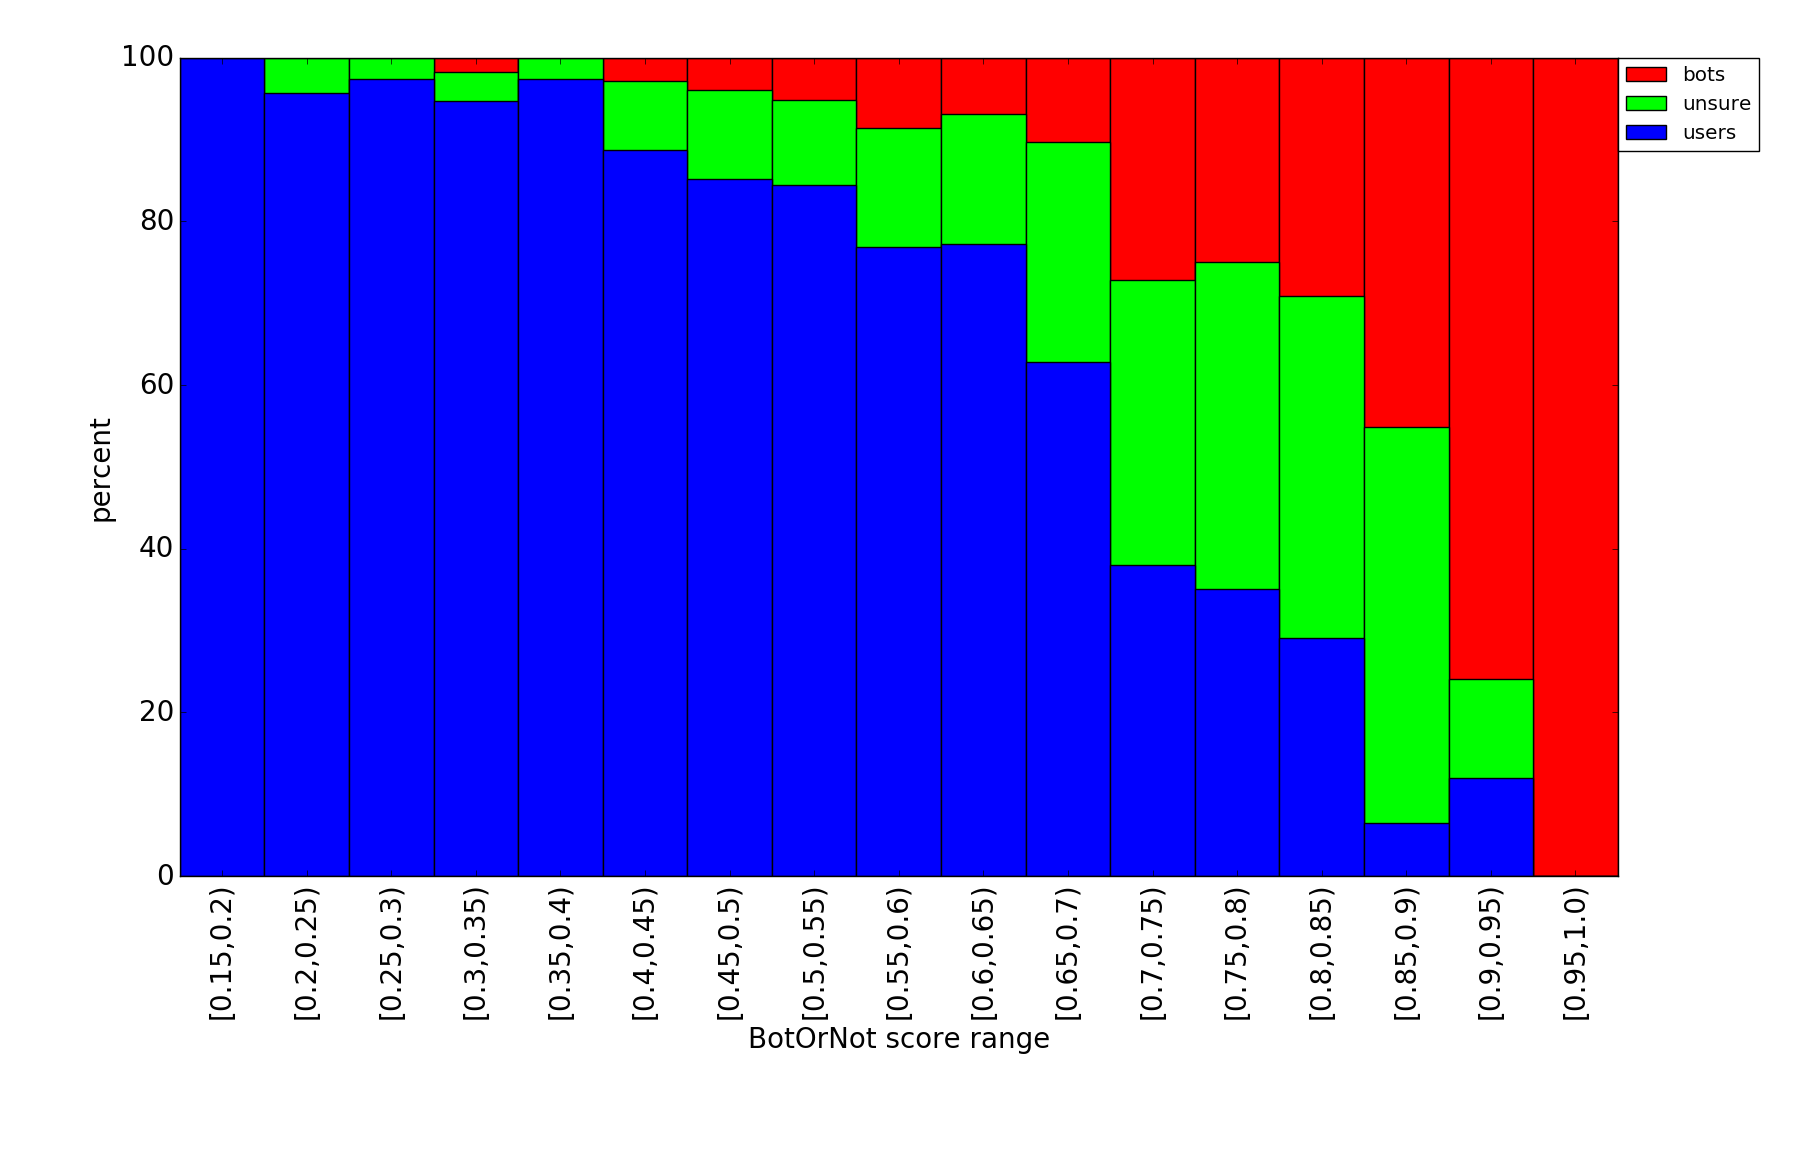
\includegraphics[width=0.4\textwidth]{imgs/scoreperc}
	\label{fig:scorescat}
	
\end{figure}

\begin{table*}
\centering
\begin{tabular}{l*{5}{c}}
Category          & [0, 20\%) & [20\%, 40\%) & [40\%, 60\%) & [60\%, 80\%) & [80\%, 100\%] \\
\hline
Human									& 10 & 150 & 277 & 204 & 21 \\
Bot            				& 0  & 1   & 17  & 70  & 53  \\
Indeterminate         & 0  & 5   & 37  & 114 & 41  \\
\end{tabular}
\caption{Number of manually classified accounts within \emph{BotOrNot} score ranges}
\end{table*}

We next examined how an account's overall \emph{BotOrNot} score aligned with the average of its corresponding category subscores, confirming that, with some deviations, the \emph{BotOrNot} score was a better predictor of whether or not a user's account was automated. From Figure \ref{fig:scoresubscore}, we see that classifying the accounts based on the overall \emph{BotOrNot} score is more effective than using the averaged category subscores.

\begin{figure}[h!]
	\caption{\emph{BotOrNot} Scores vs Category Subscores}
	\centering
		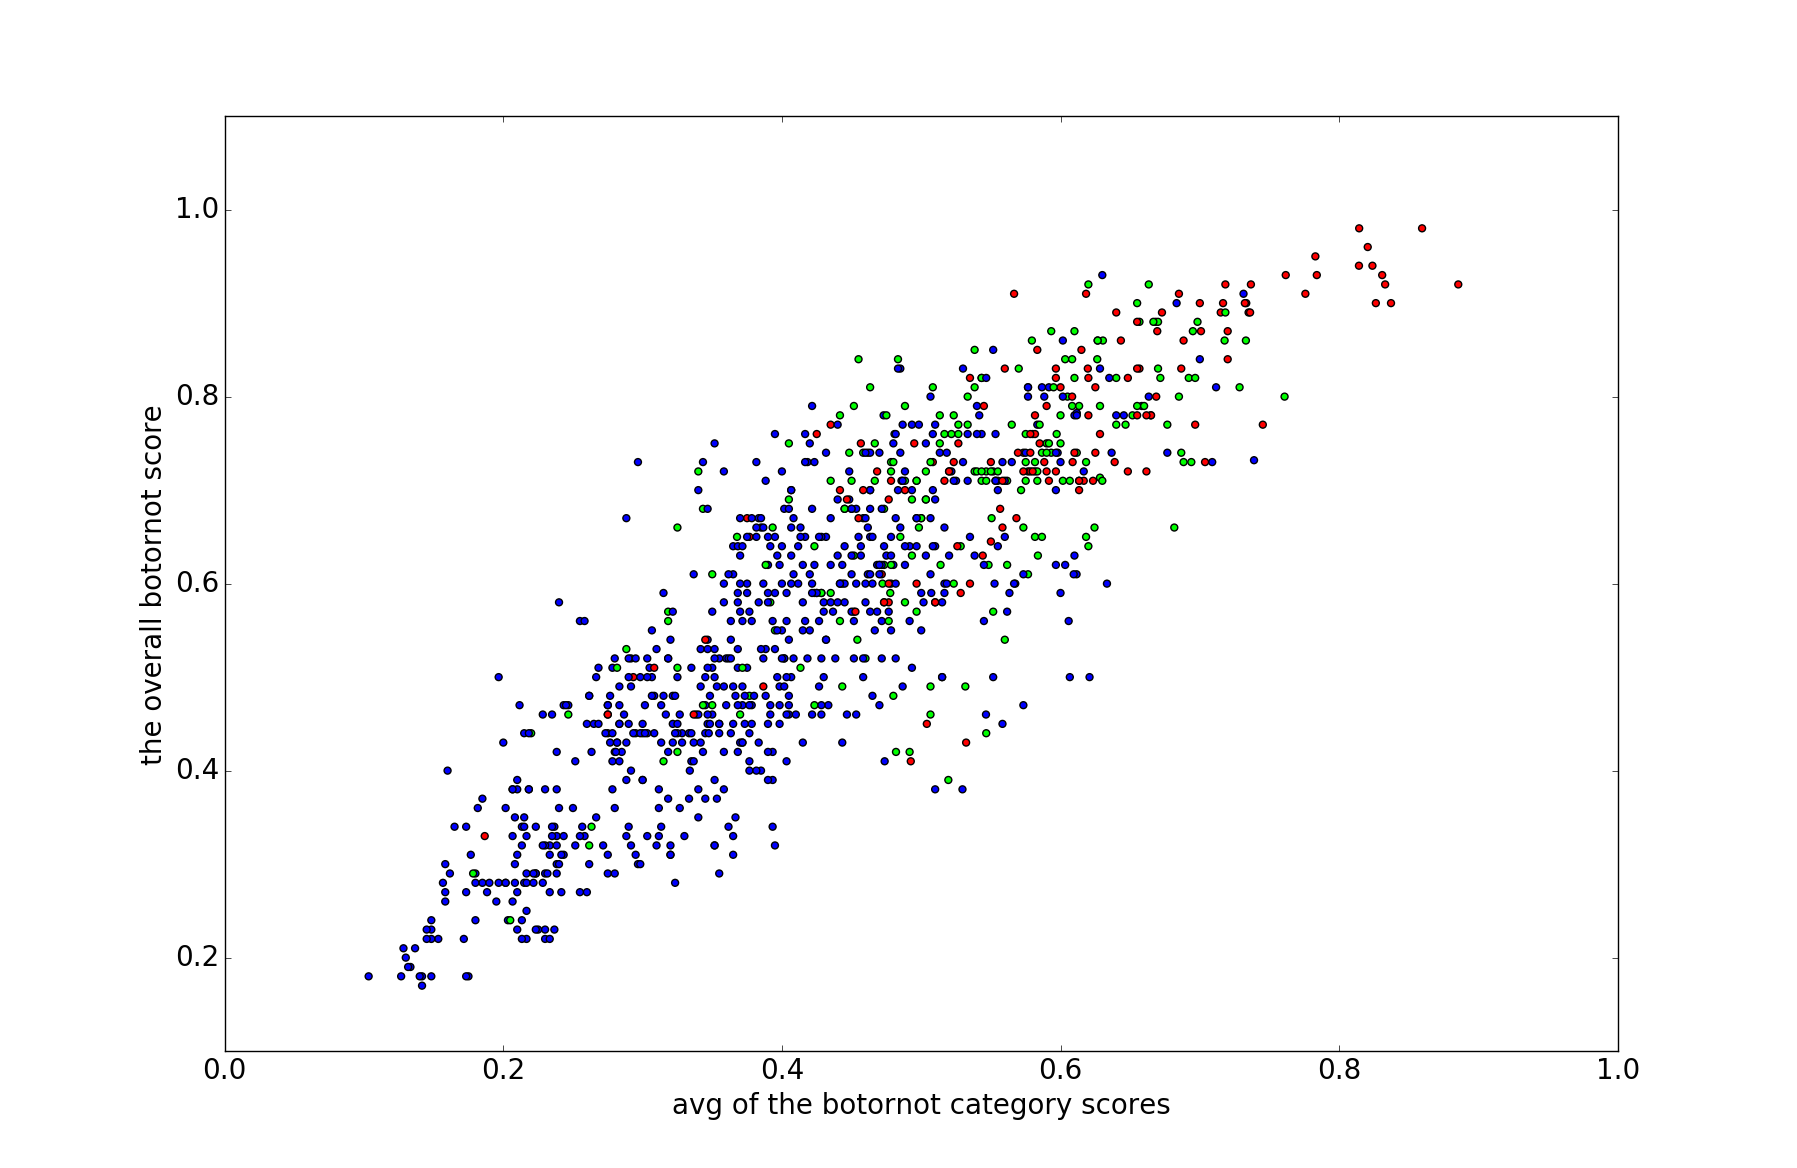
\includegraphics[width=0.5\textwidth]{imgs/svacs}
	\label{fig:scoresubscore}
\end{figure}

Our unsupervised machine learning algorithms were able to similarly separate bot users and human users, as seen in Figure \ref{fig:clustscore}. Clusters are visible on the same horizontal line, and these clusters tend to be either mainly bots or mainly humans.

\begin{figure}[h!]
	\caption{\emph{BotOrNot} Clustering vs Average Scores}
	\centering
		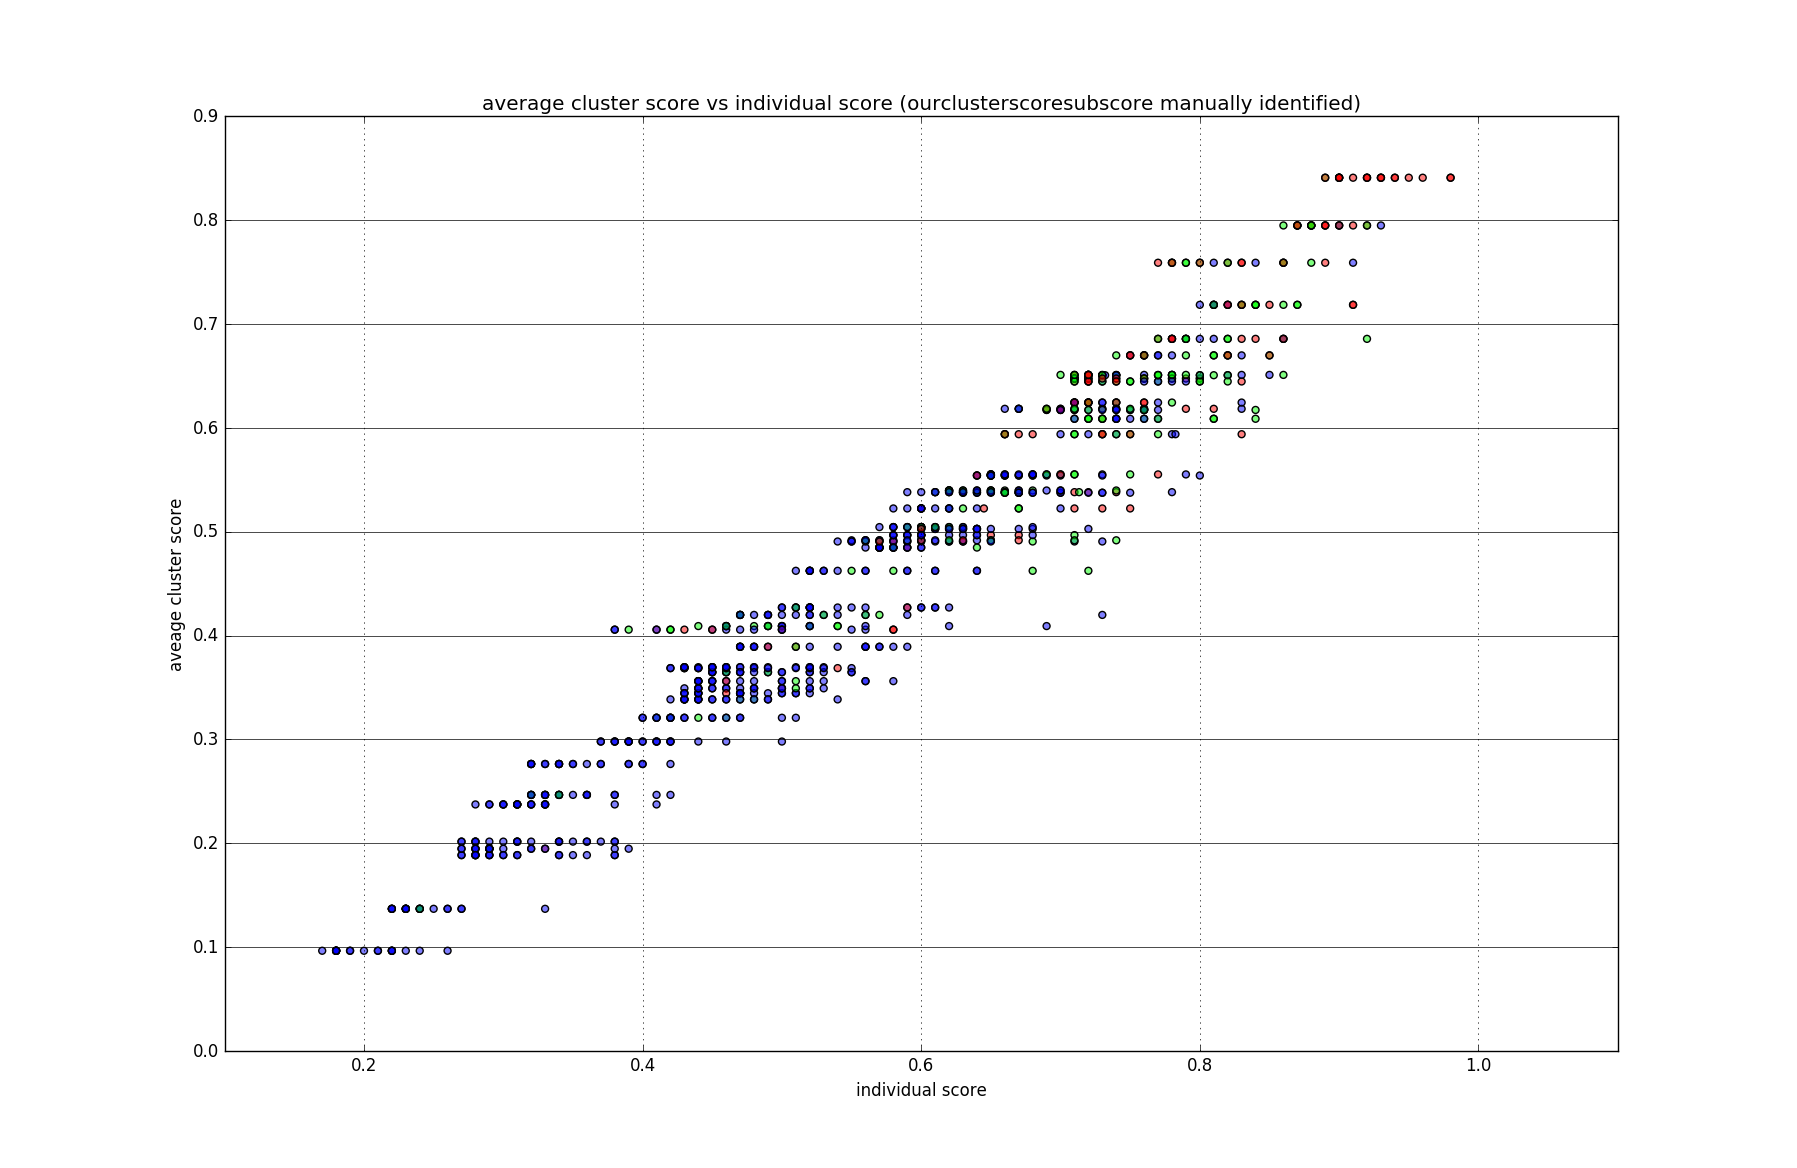
\includegraphics[width=0.5\textwidth]{imgs/ourscorevssubscore}
	\label{fig:clustscore}
\end{figure}

\subsection{Mentions}
As seen in Figure \ref{fig:ment1}, we found that Twitter bots tended to not mention specific users, with most bot clusters having fewer than 17 mentions per user. Twitter's guidelines for bots are particularly explicit about this aspect of the service:

\begin{quote}If your application creates or facilitates automated reply messages or mentions to many users, the recipients must request or otherwise indicate an intent to be contacted in advance.\cite{twitter:automation}\end{quote}

In Figure \ref{fig:ment2}, we examine the amount that accounts in clusters that mention users actually do so. If bots tended towards a similar rate of mentioning users as humans did, we would expect to see the data remain similar across clusters from Figure \ref{fig:ment1} to Figure \ref{fig:ment2}. However, since bots tend to mention at a higher frequency when they do mention other users, clusters containing bots have comparatively higher mentioning rates in Figure \ref{fig:ment2}. In clusters of humans, the mentioning characteristics of those users is more uniform. In contract, in the bot clusters, automated accounts tend to have either a medium amount of mentions, or none at all.

\begin{figure}[h!]
	\caption{Mentions Per Cluster}
	\label{fig:ment1}
	\centering
		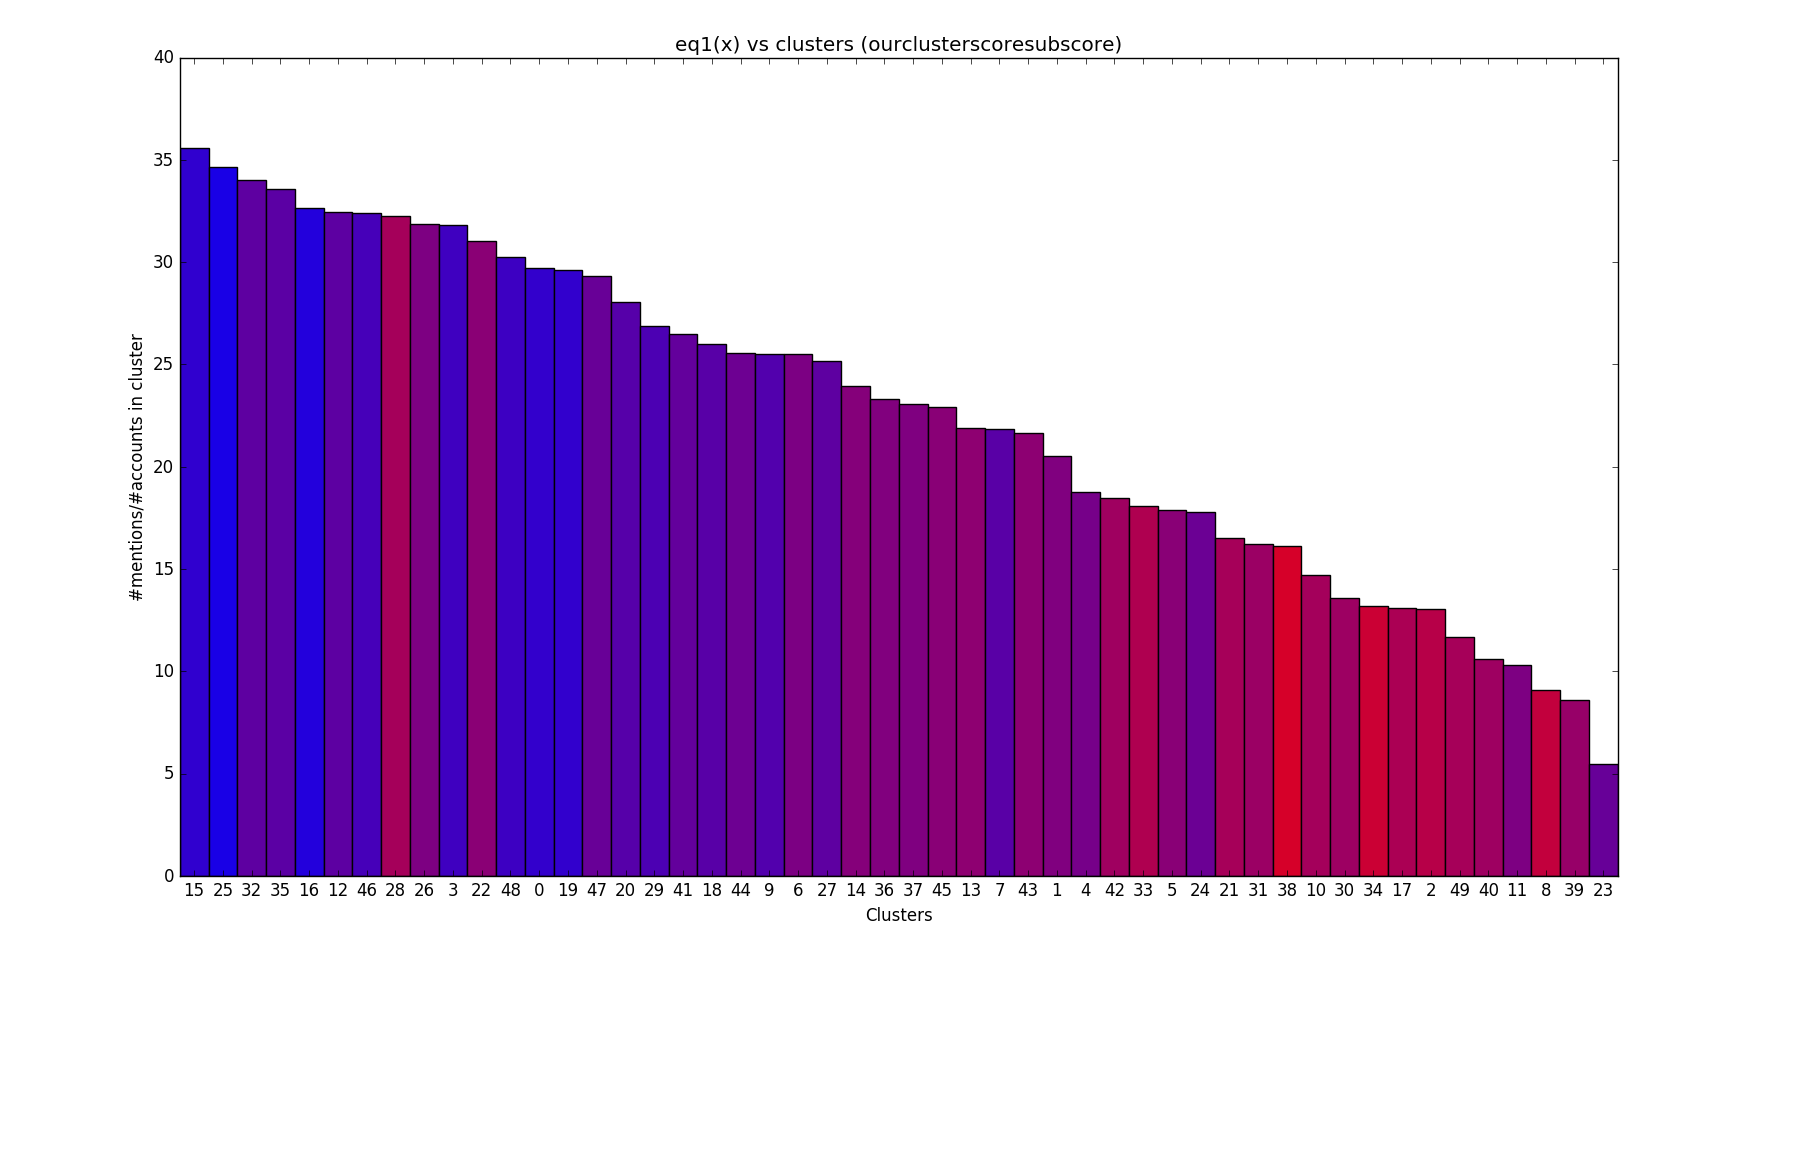
\includegraphics[width=0.5\textwidth]{imgs/mentionspercluster}
\end{figure}

\begin{figure}[h!]
	\caption{Mentions Per User}
	\label{fig:ment2}
	\centering
		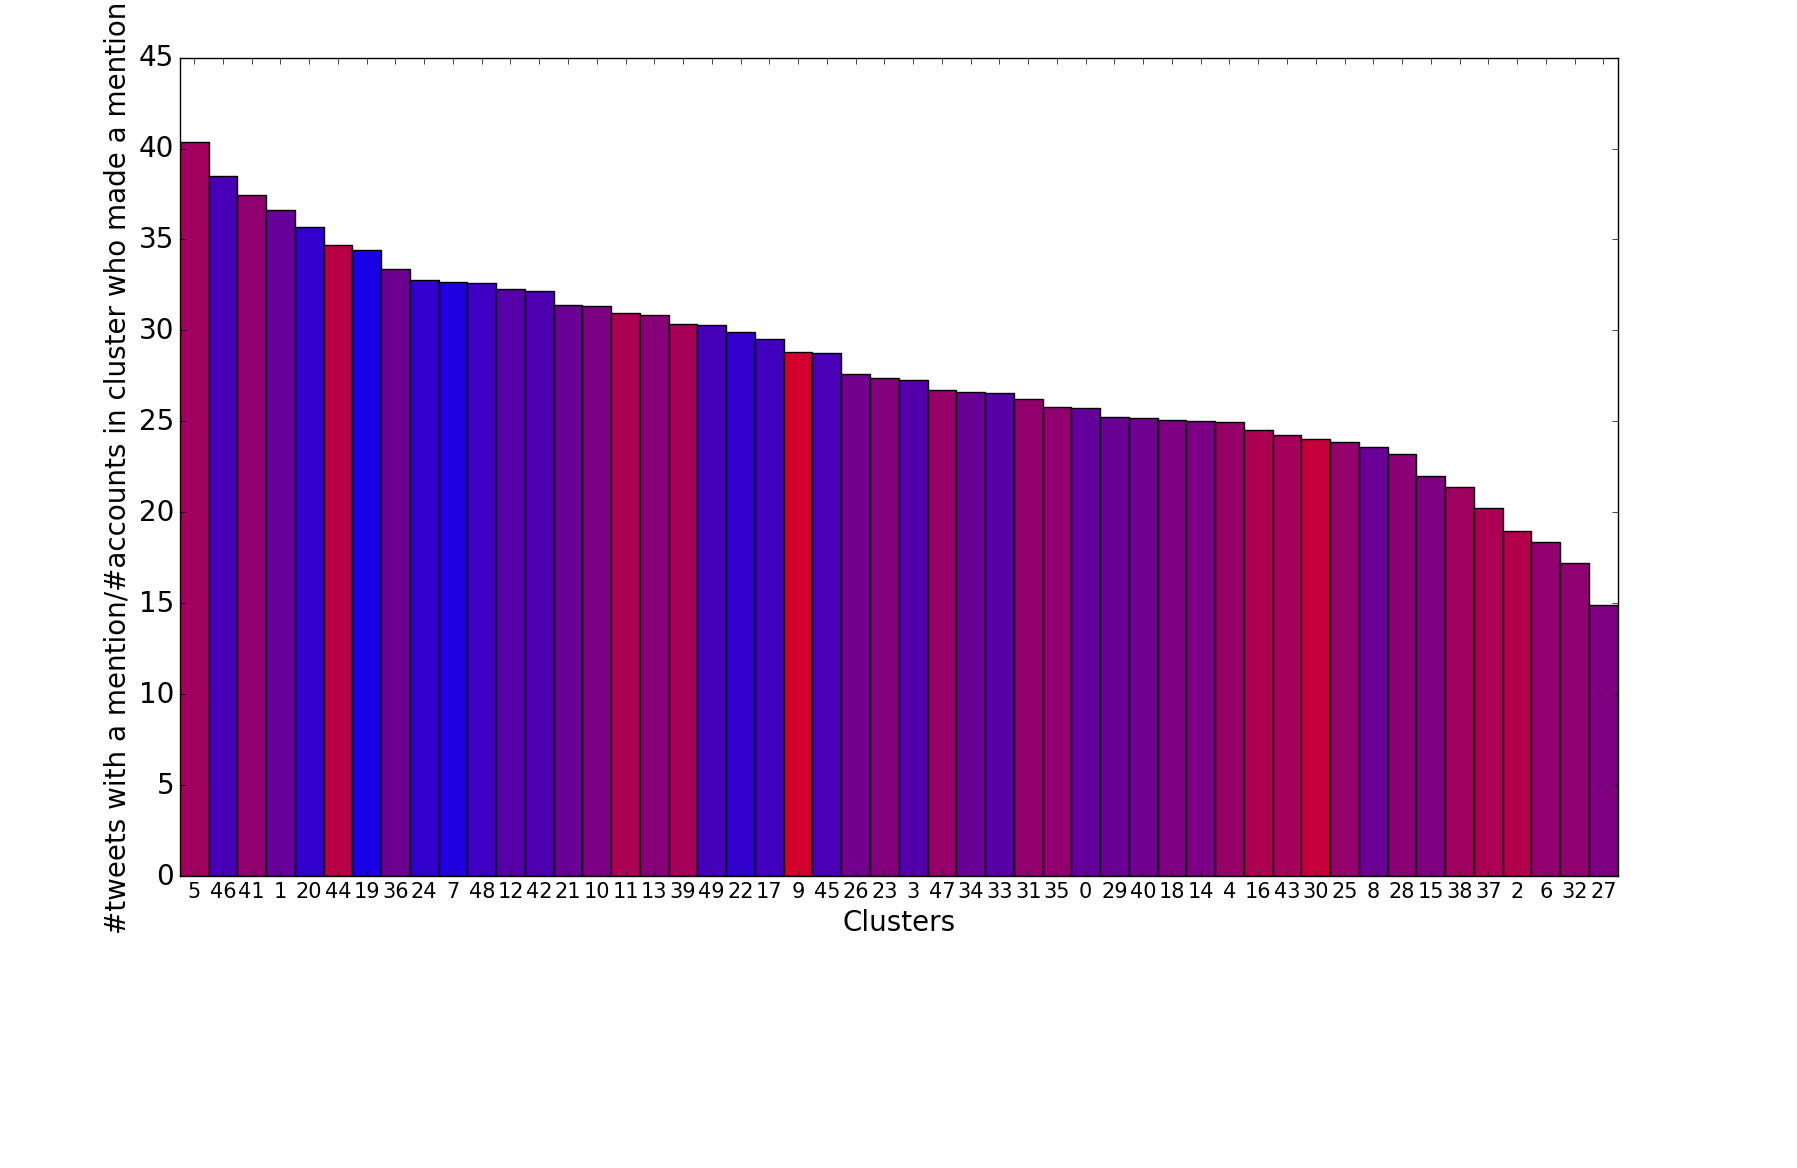
\includegraphics[width=0.5\textwidth]{imgs/mentionsperuserpercluster}
\end{figure}

\subsection{Retweets}

Similar to automated mentions, Twitter's guidelines explicitly forbid automated retweeting:

\begin{quote}Automation of Retweets often leads to spam and other negative user experiences; therefore, Retweeting in a bulk or automated manner is prohibited.\cite{twitter:automation}\end{quote}

Very few users classified as bots mention other users or retweet their tweets, which indicates that Twitter is closely monitoring these methods of user interaction; either very few bots are being created to automate these actions or they are rapidly banned from the service.

\begin{figure}[h!]
	\caption{RTs Per Cluster}
	\centering
		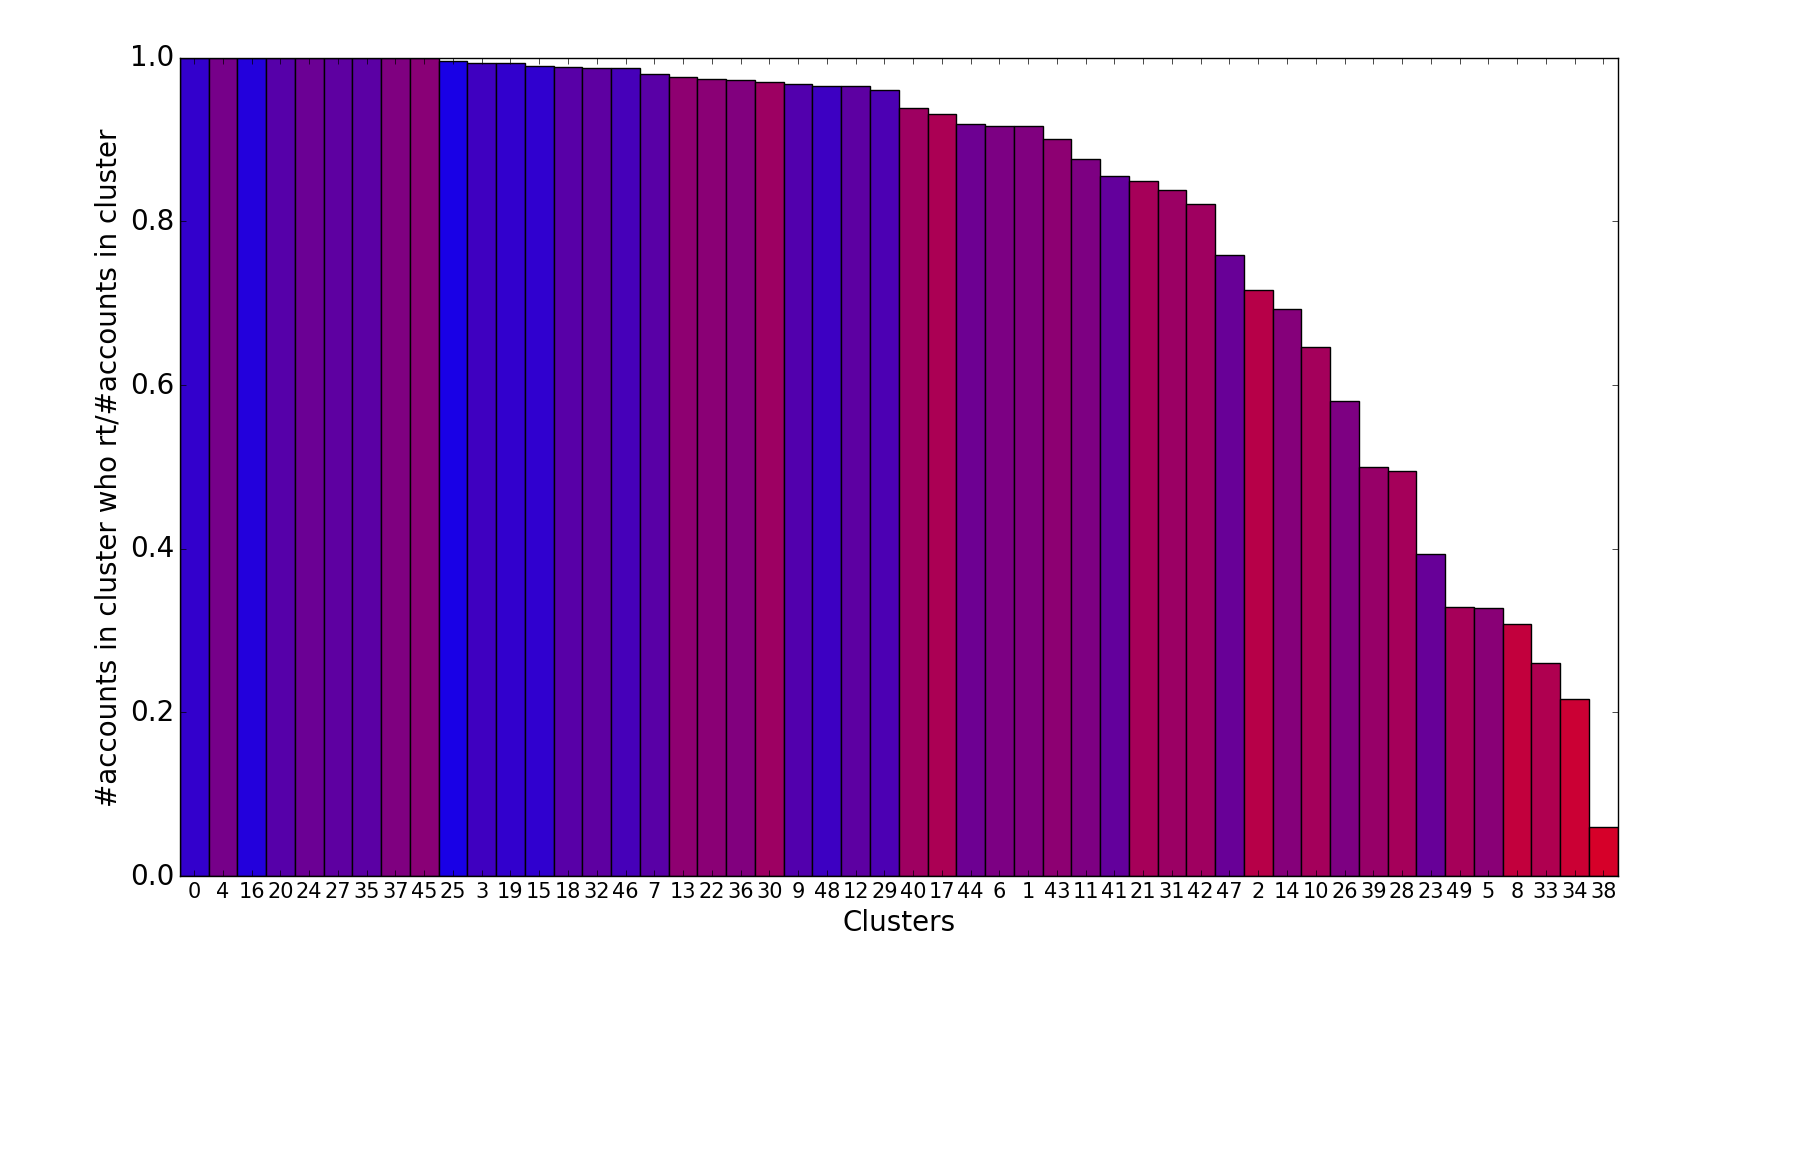
\includegraphics[width=0.5\textwidth]{imgs/rt3}
\end{figure}

\subsection{Hashtags}

Due to some selection bias for the Twitter accounts we scanned, a disproportionate number of users tweeted using hashtags related to a shared interest, such as independent game development.

However, examining how many times each user in a cluster used a hashtag, as shown in Figure \ref{fig:hsh}, gave a more indicative view of hashtags used for spamming, such as ``fifa15coins'' and a number of sexually explicit hashtags. Many of these spammed hashtags were only tweeted by a single user, which indicates that the creators of these spam accounts attempt to avoid overlap in which hashtags they are spamming. While Twitter's terms of service forbids automatically posting into the trending topics, it does not forbid automation using hashtags, allowing for these bots to find commonly popular hashtags and spam them without much apparent risk.

A large number of users tweeted with the hashtag of ``Finances,'' but under further inspection a majority of these accounts were verified, indicating that while these accounts may exhibit spamming behavior, they were likely controlled by humans.

\begin{figure*}[h!]
	\caption{Hashtags Per User}
	\centering
		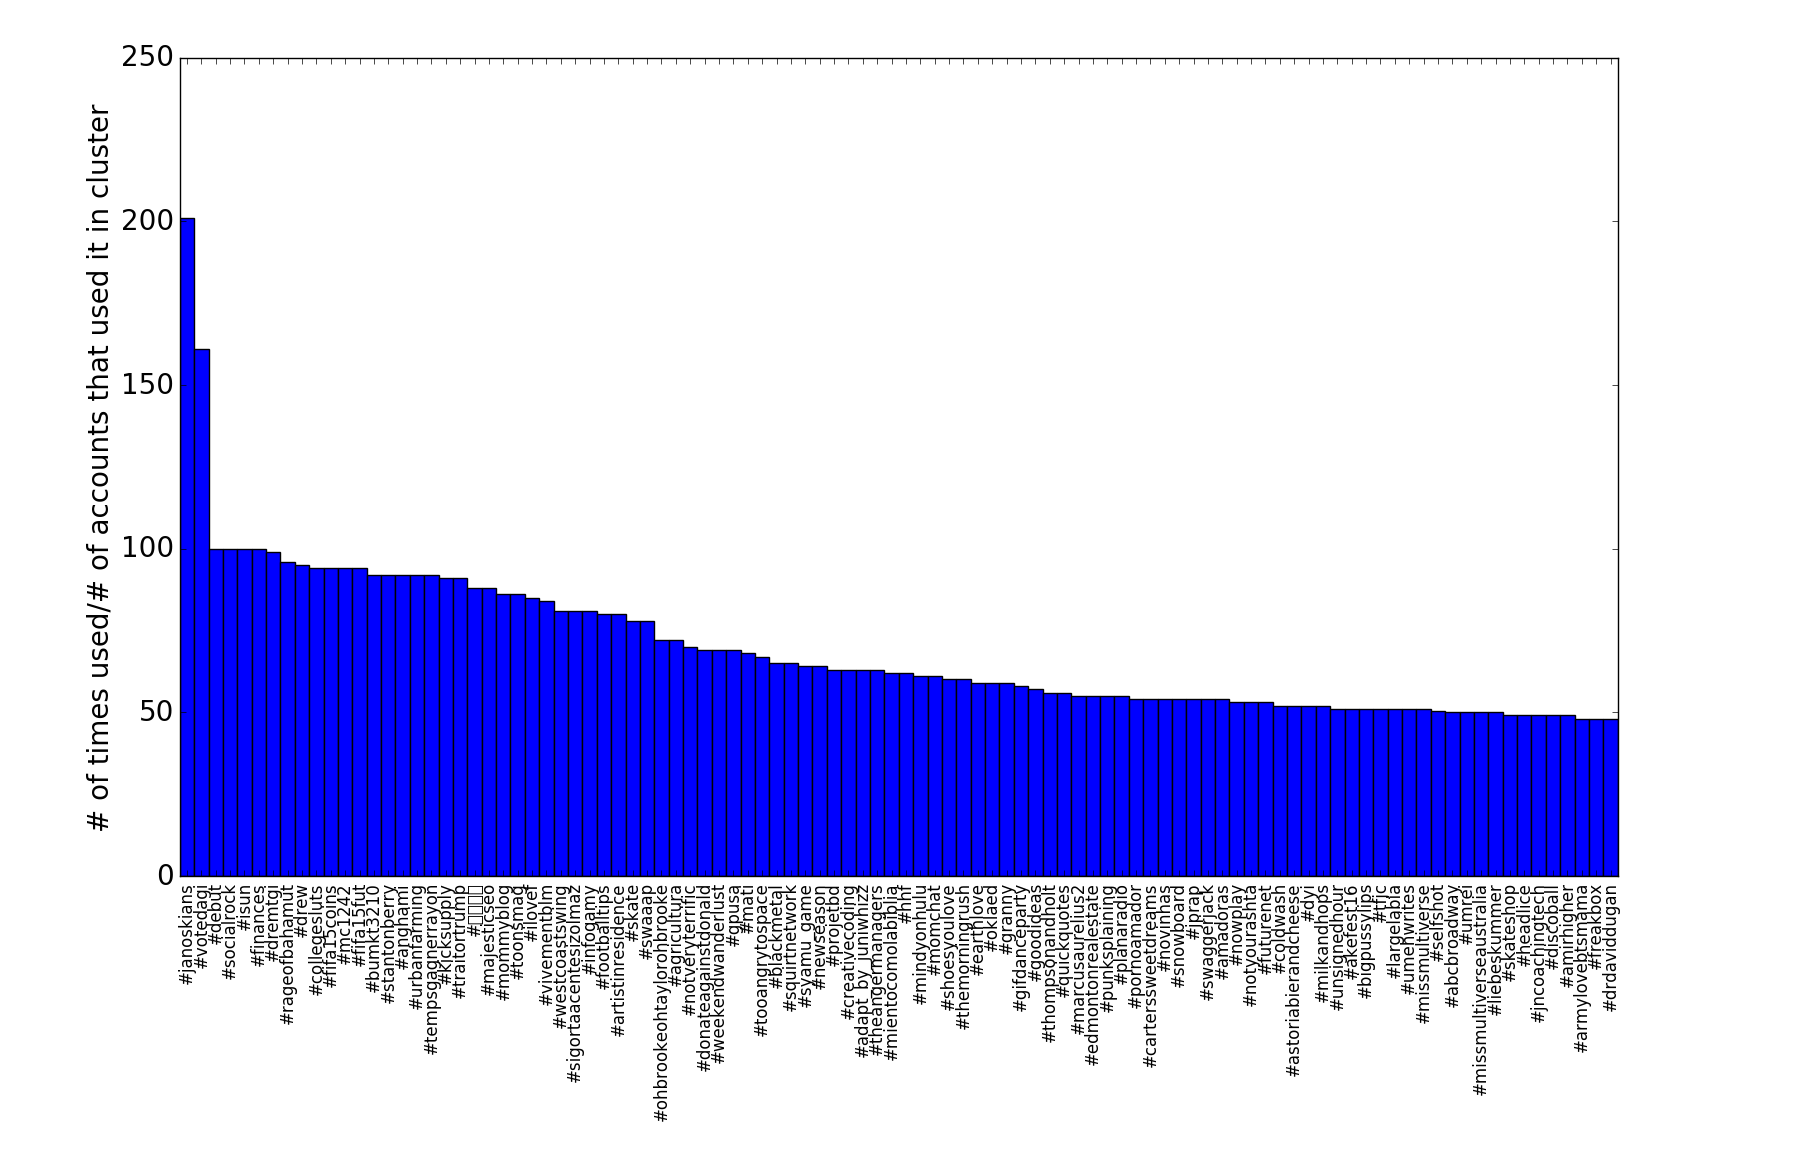
\includegraphics[width=0.95\textwidth]{imgs/bhvc}
	\label{fig:hsh}
\end{figure*}

Examining a cluster comprised mainly of bots, such as cluster 33 in Figure \ref{fig:hsh33}, confirms that these automated users are far more likely to repeatedly use the same sexually explicit hashtags, in addition to very general hashtags such as ``NBA.''

\begin{figure*}[h!]
	\caption{Hashtags Per User (Cluster 33)}
	\centering
		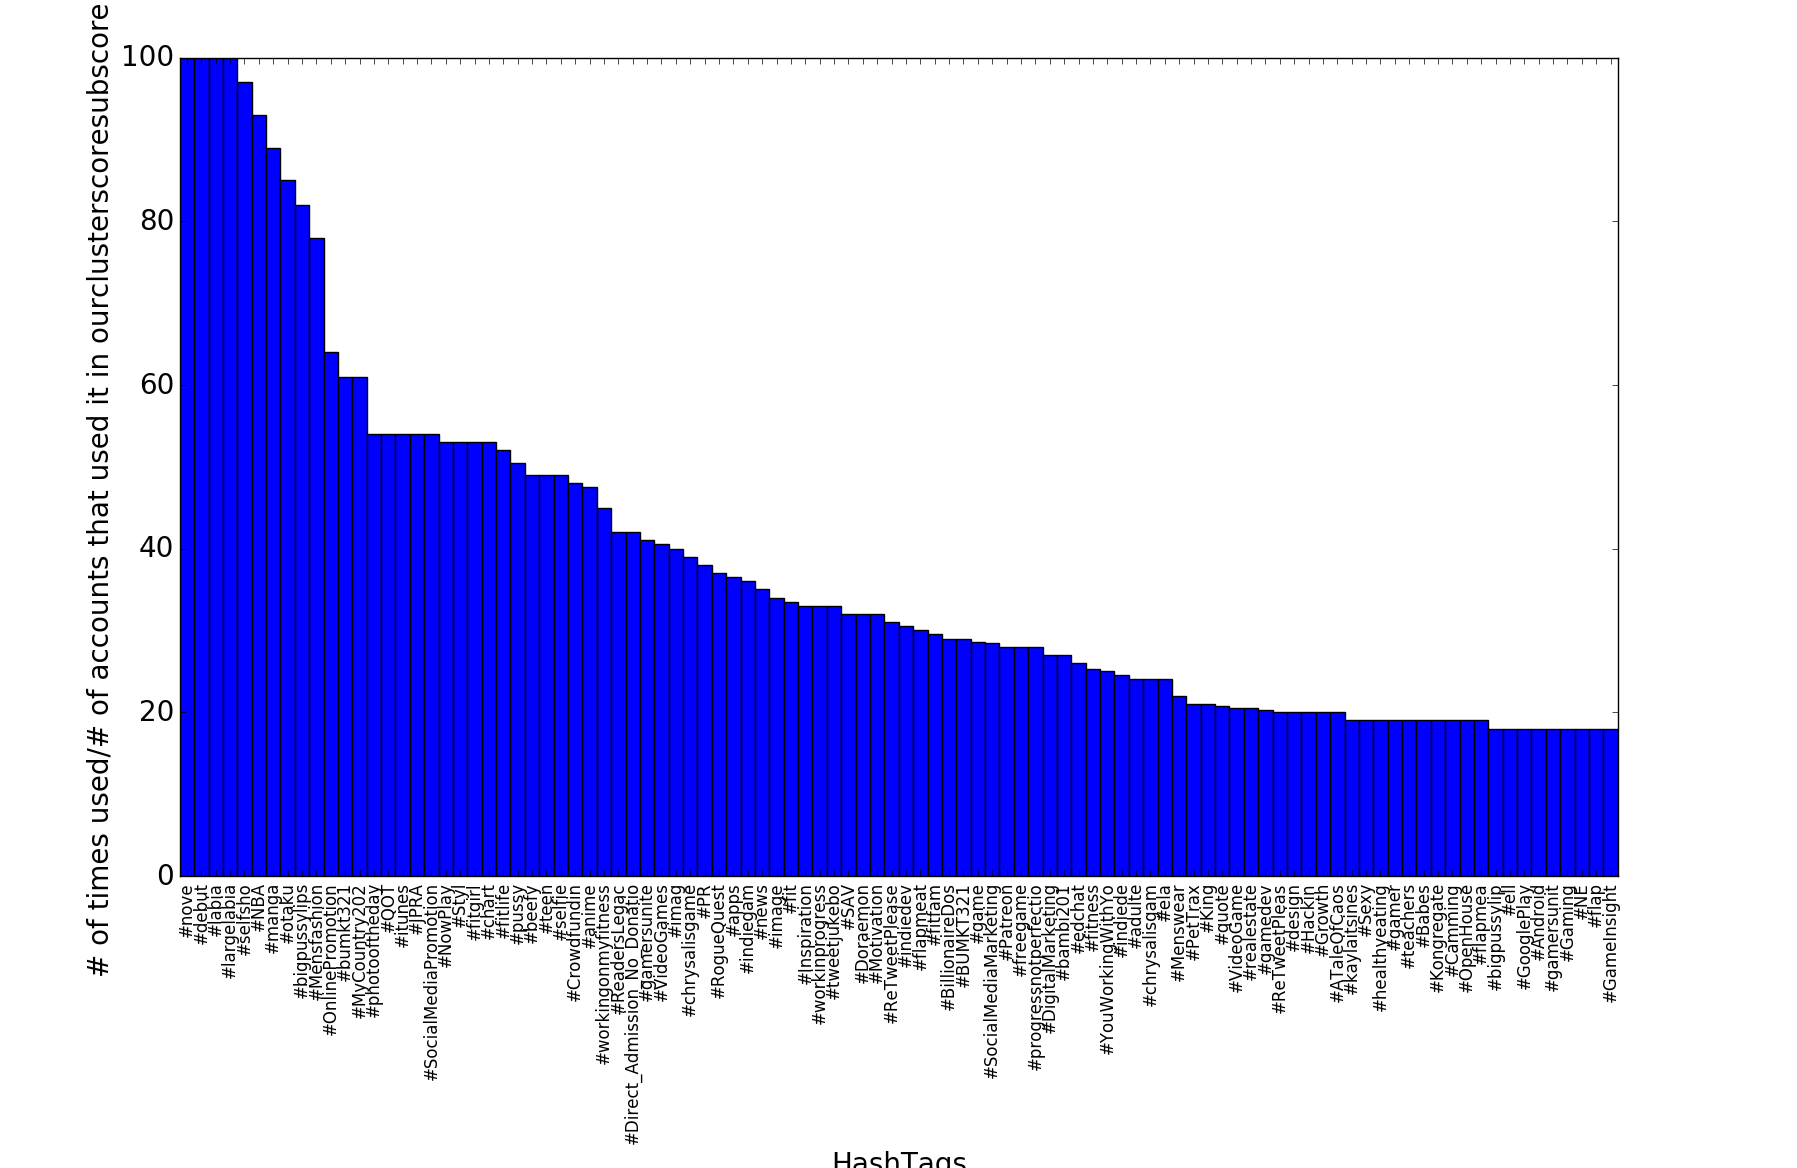
\includegraphics[width=0.95\textwidth]{imgs/bhvc33}
	\label{fig:hsh33}
\end{figure*}

\subsection{Following}

While Twitter forbids automated following, it's one of the most common methods bots use to gain attention from human users. Most bots are following over 10,000 users; they also have similarly exaggerated numbers of followers.

We noticed one cluster of users sharing an extremely large number of both followers and accounts they followed; upon further inspection, the majority of these accounts were promotional accounts. Since they tend to follow back, these accounts become a prime target for sockpuppet accounts that want to appear legitimate; both the following and follower tabs are filled with users who have the default Twitter profile picture and no tweets, with many of their creation dates within the last month.

\begin{figure}[h!]
	\caption{Following Per Cluster}
	\centering
		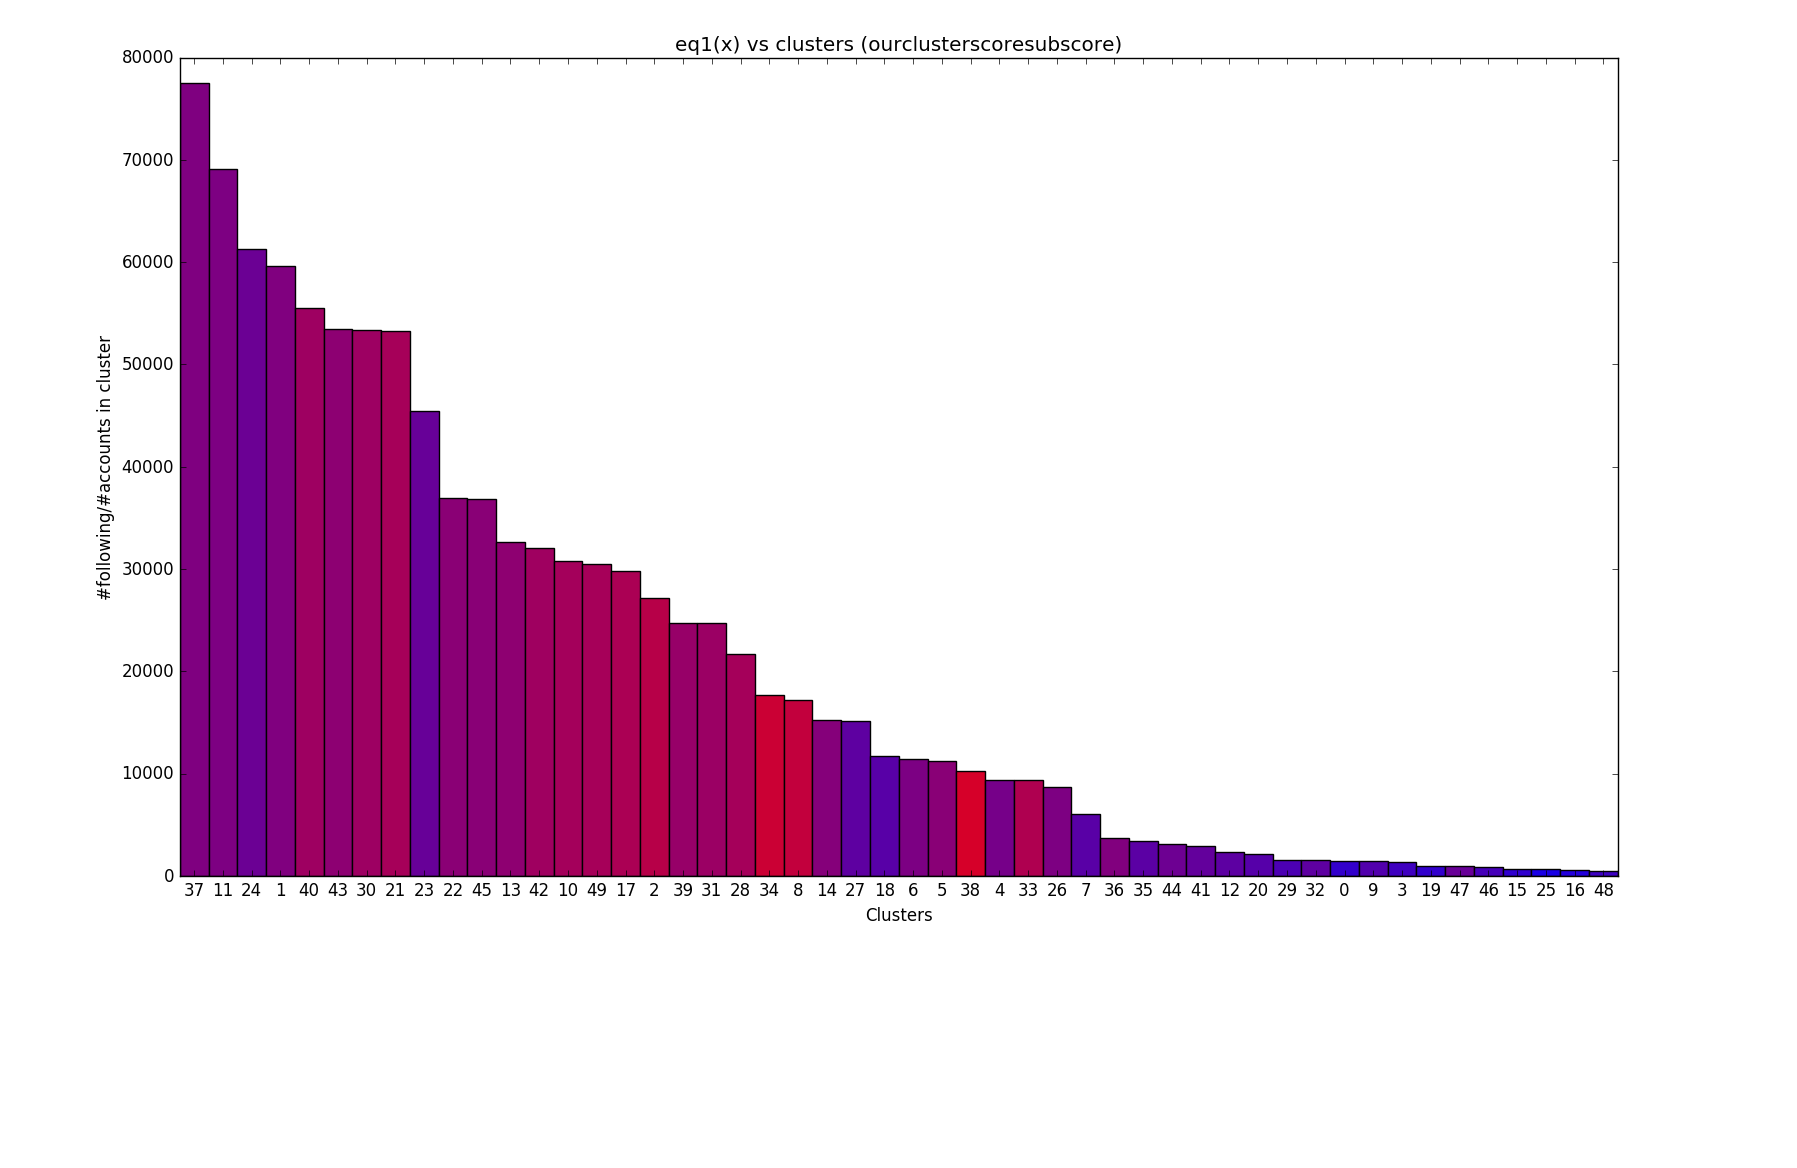
\includegraphics[width=0.5\textwidth]{imgs/following}
\end{figure}

\subsection{Favoriting}

Examining how often users favorited tweets gave an interesting trend; bots tended to either favorite very few tweets, or a very large number of them, with human users hovering in between the two extremes.

We manually examined the users in clusters 22 and 33. Cluster 22 had the largest number of favorites, while cluster 33 favorited a large number of tweets and scored rather heavily in the \emph{BotOrNot} assessment. Cluster 22 was comprised mainly of businesses and other Twitter ``personalities'' such as YouTubers. These users likely either search their names and favorite tweets including that text, or favorite the tweets that mention them as a way of quickly responding to fans.

Cluster 33, however, was comprised of accounts that tweeted links to related sites with little commentary besides relevant hashtags. These ``aggregator'' Twitter accounts search for hashtags and tweets relating to the topic that they post and then favorite those tweets. This behavior may pass under Twitter's radar because the accounts select phrases to search for that are relatively uncommon, simply reflecting the intermittent behavior of other users.

\begin{figure}[h!]
	\caption{Favorites Per Cluster}
	\centering
		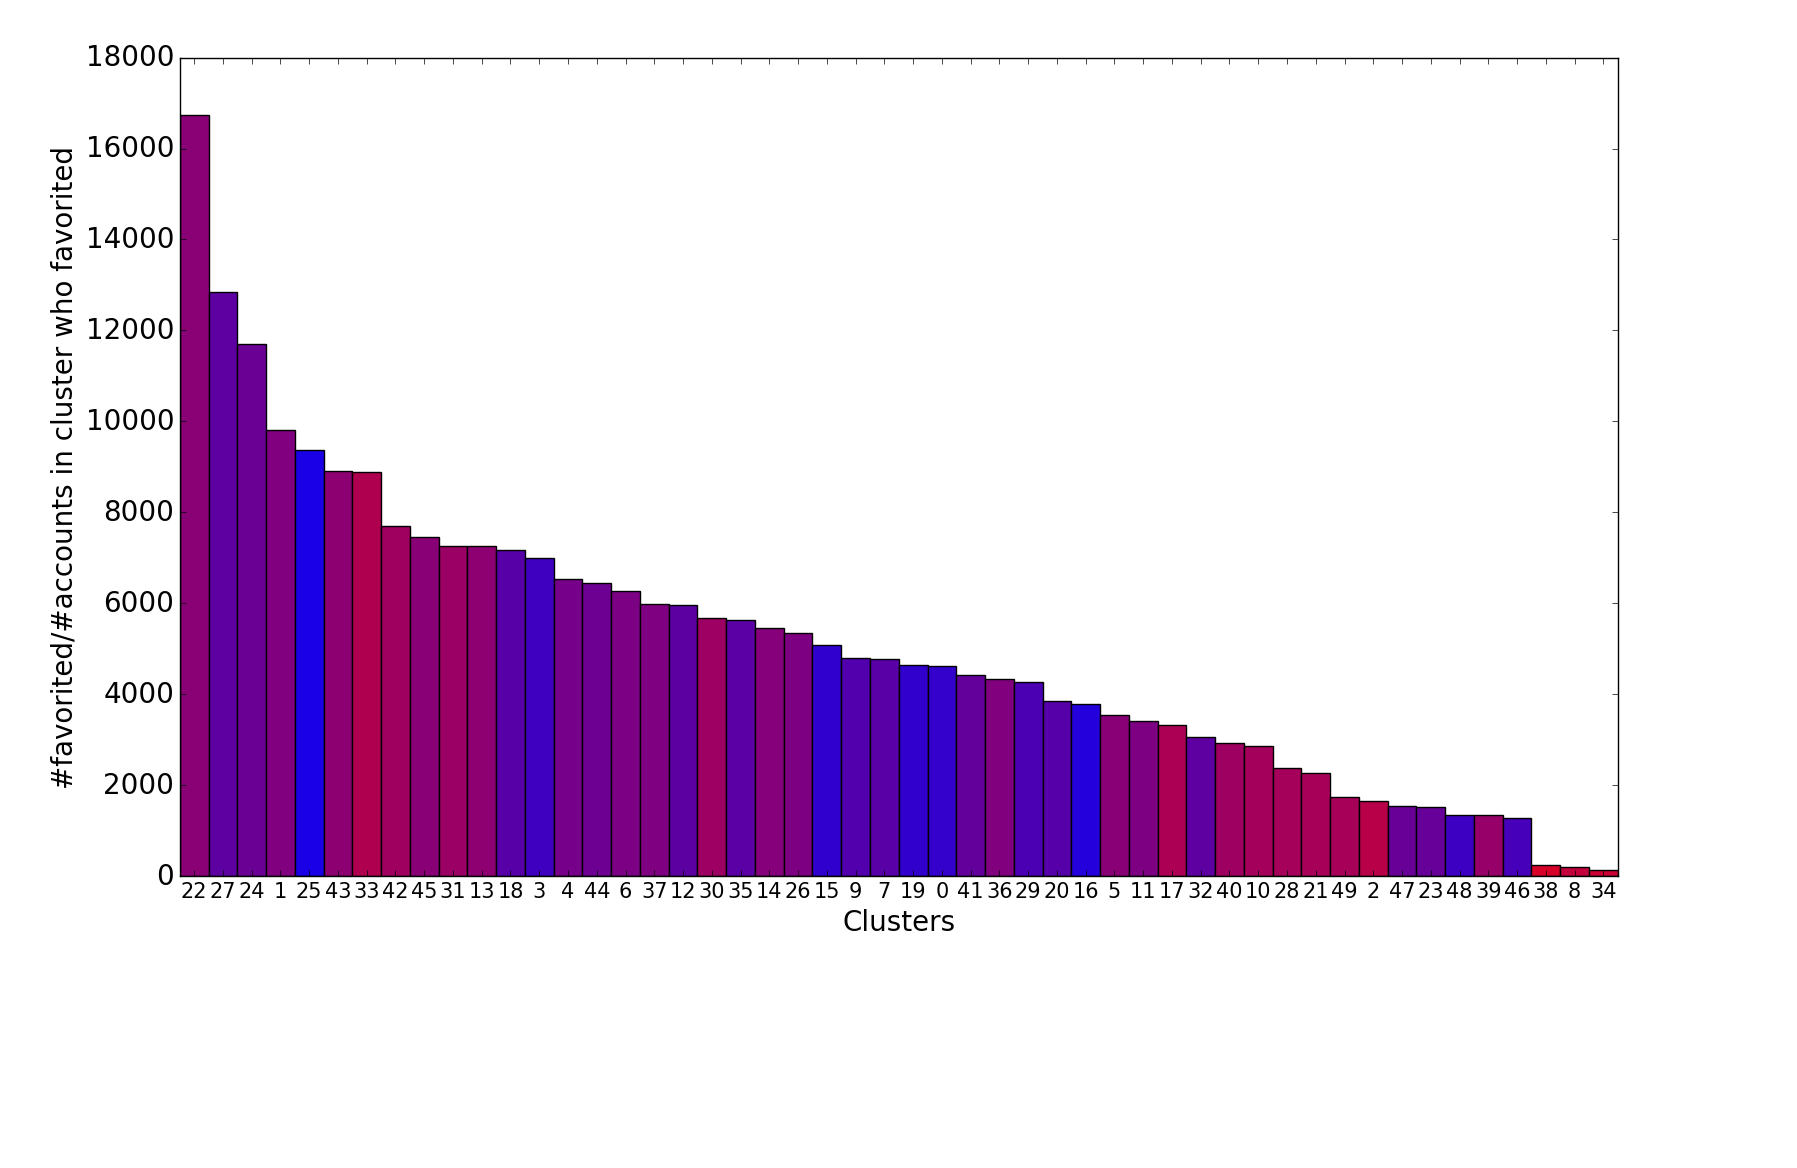
\includegraphics[width=0.5\textwidth]{imgs/favorites}
\end{figure}

\section{Conclusion}
% CONCLUSION (~1/4 pages)
Our study focused on analyzing interaction between human and bot Twitter users. We used \emph{BotOrNot}, combined with unsupervised machine learning, to cluster users and determine how bots gain visibility with their target audience. We determined that bots are generally unlikely to engage with human users beyond simply following them and using hashtags. However, when bots \emph{do} interact with users, they do so without moderation, resulting in bots tending towards behavioral extremes.

\subsection{Further Work}
Although we were able to manually identify advertising links, when we retrieved data on individual Tweets we did not expand Twitter's shortened URL format. This made media, such as photos, appear identical to other links, since Twitter represents media as URLs. In addition, the sample size for manual classification was small by necessity; setting up a web service such as Mechanical Turk to crowdsource this account classification would improve analysis and clustering.

Furthermore, while several accounts were discovered that exhibited bot-like behavior such as spamming a hashtag, a number of these accounts were verified by Twitter, especially those run by so-called ``financial consultants.'' While a closer examination of these users was outside the scope of this project, they seem closely related to the issue of spambots, and further discussion as to whether these accounts violate Twitter's terms of service seems warranted.

While we sought to provide an analytical overview of our sample users, a deeper statistical analysis of individual clusters and bots is warranted, based on several of the characteristics we identified. In particular, analyzing the distribution of mentions across individual clusters of bots and clusters of humans would lead to greater insight into that aspect of their behavior.

Finally, Twitter allows for users to quote other Tweets, as a commentary layered upon a retweet. This is unlikely to be a vector by which bots interact with humans, but it would provide a further view of Twitter users' behavioral patterns and its absence could possibly indicate automated behaviors.

%
% The following two commands are all you need in the
% initial runs of your .tex file to
% produce the bibliography for the citations in your paper.
\bibliographystyle{abbrv}
\bibliography{sigproc}  % sigproc.bib is the name of the Bibliography in this case
% You must have a proper ".bib" file
%  and remember to run:
% latex bibtex latex latex
% to resolve all references
%
% ACM needs 'a single self-contained file'!
%
%APPENDICES are optional
%\balancecolumns
% \appendix

\appendix
\section{Contributions}
Alic Szecsei provided data retrieval methods for Twitter accounts, programmed the unsupervised machine learning, and wrote the data analysis.

Willem DeJong programmed BotOrNot score retrieval, crawled Twitter accounts to store retrieved data in SQL databases, created many of the graphs and charts, and performed the manual account classification.

\section{Misc. Data}

\begin{figure}[h!]
	\caption{Manual identification of accounts}
	\centering
		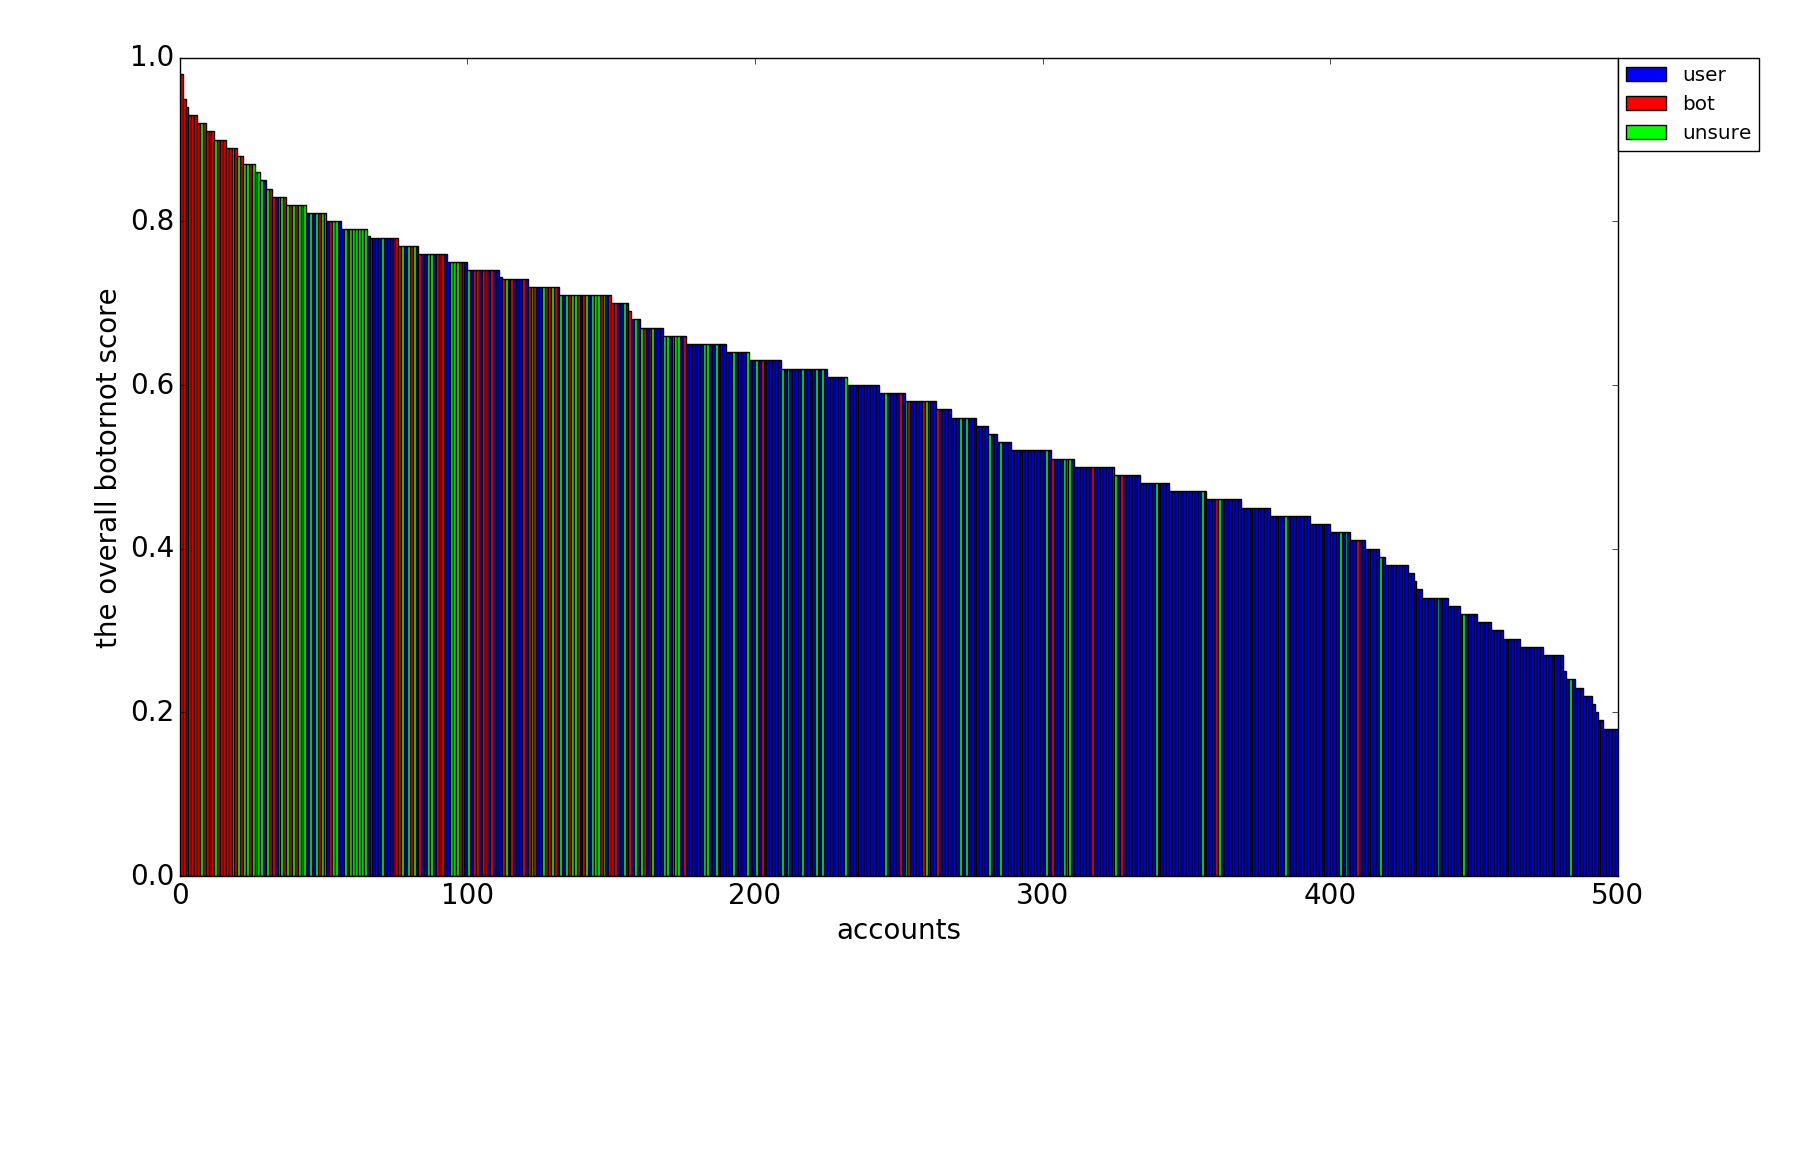
\includegraphics[width=0.5\textwidth]{imgs/barvsaccnt}
	\label{fig:barvsaccnt}
\end{figure}

\begin{figure}[h!]
	\caption{Followers Per Cluster}
	\centering
		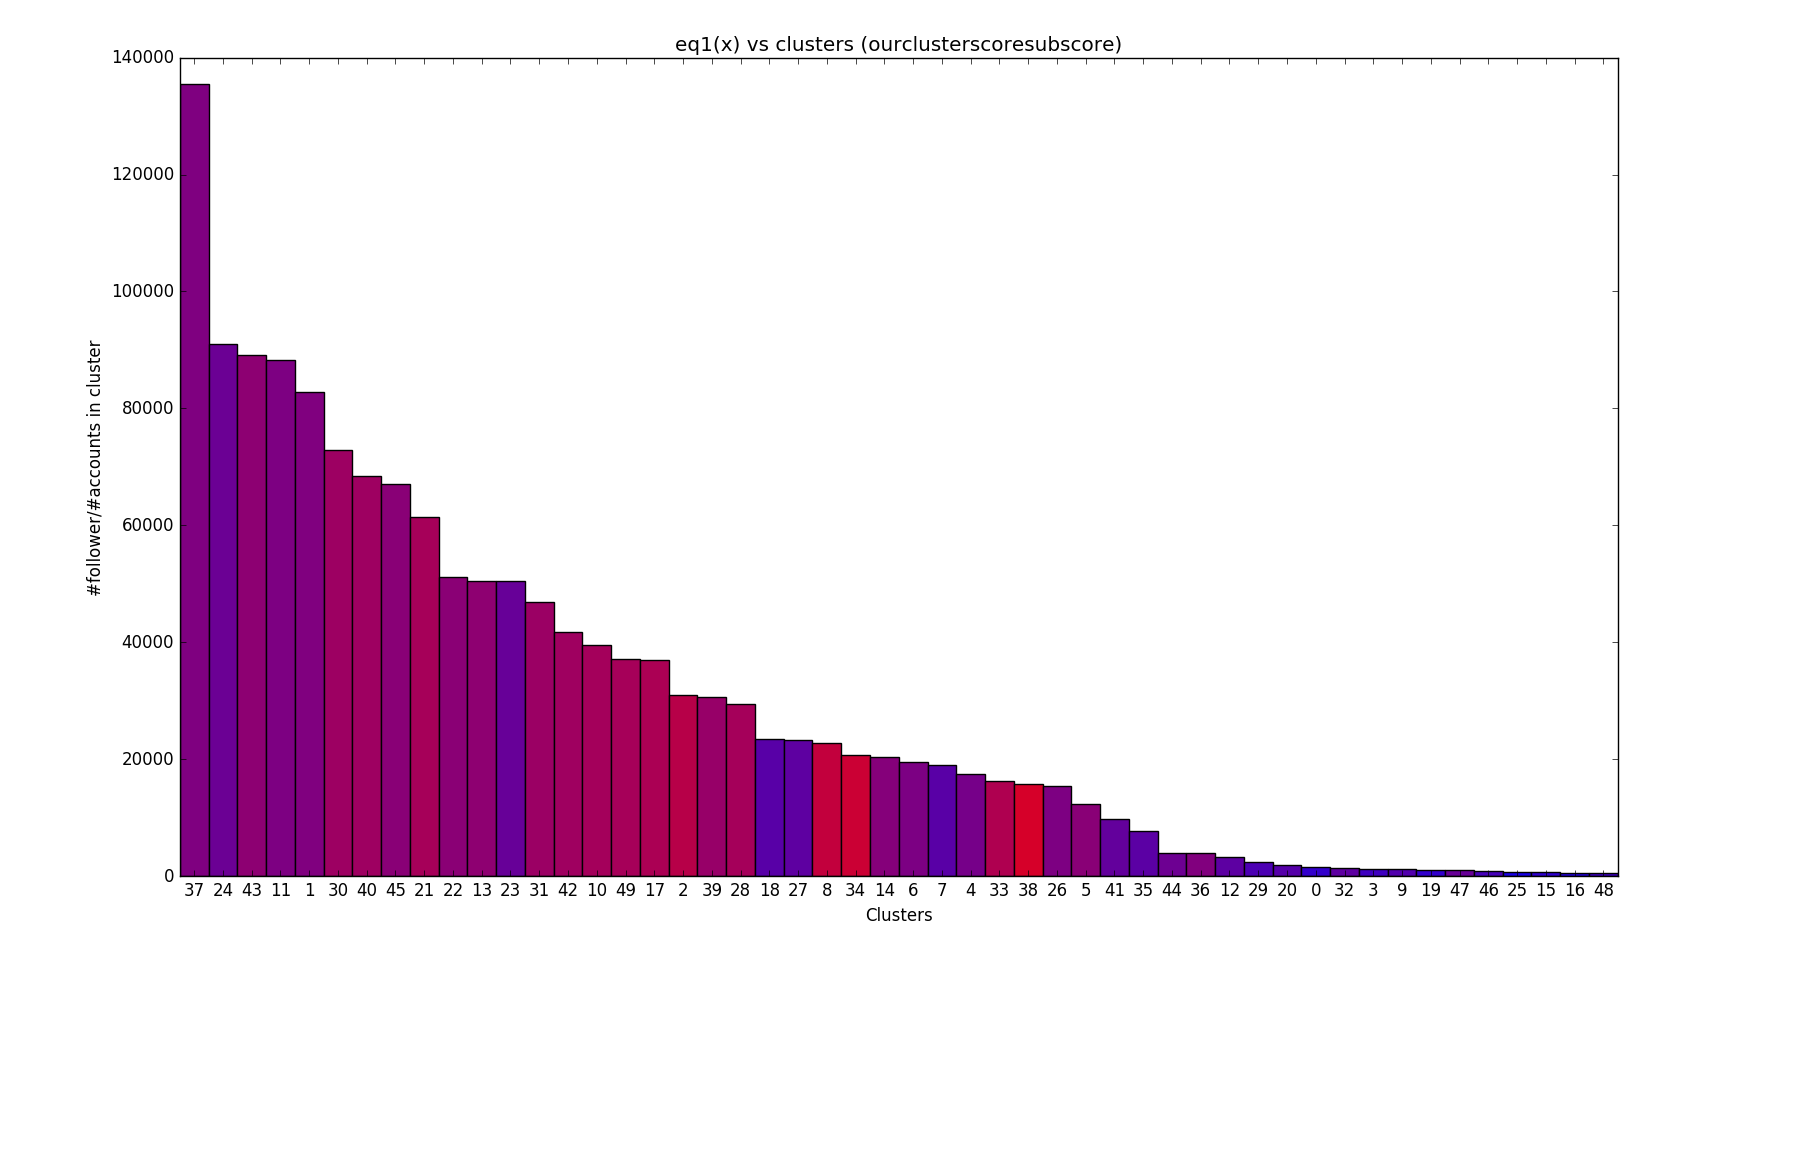
\includegraphics[width=0.5\textwidth]{imgs/followers}
\end{figure}

\begin{figure}[h!]
	\caption{Times Listed Per Cluster}
	\centering
		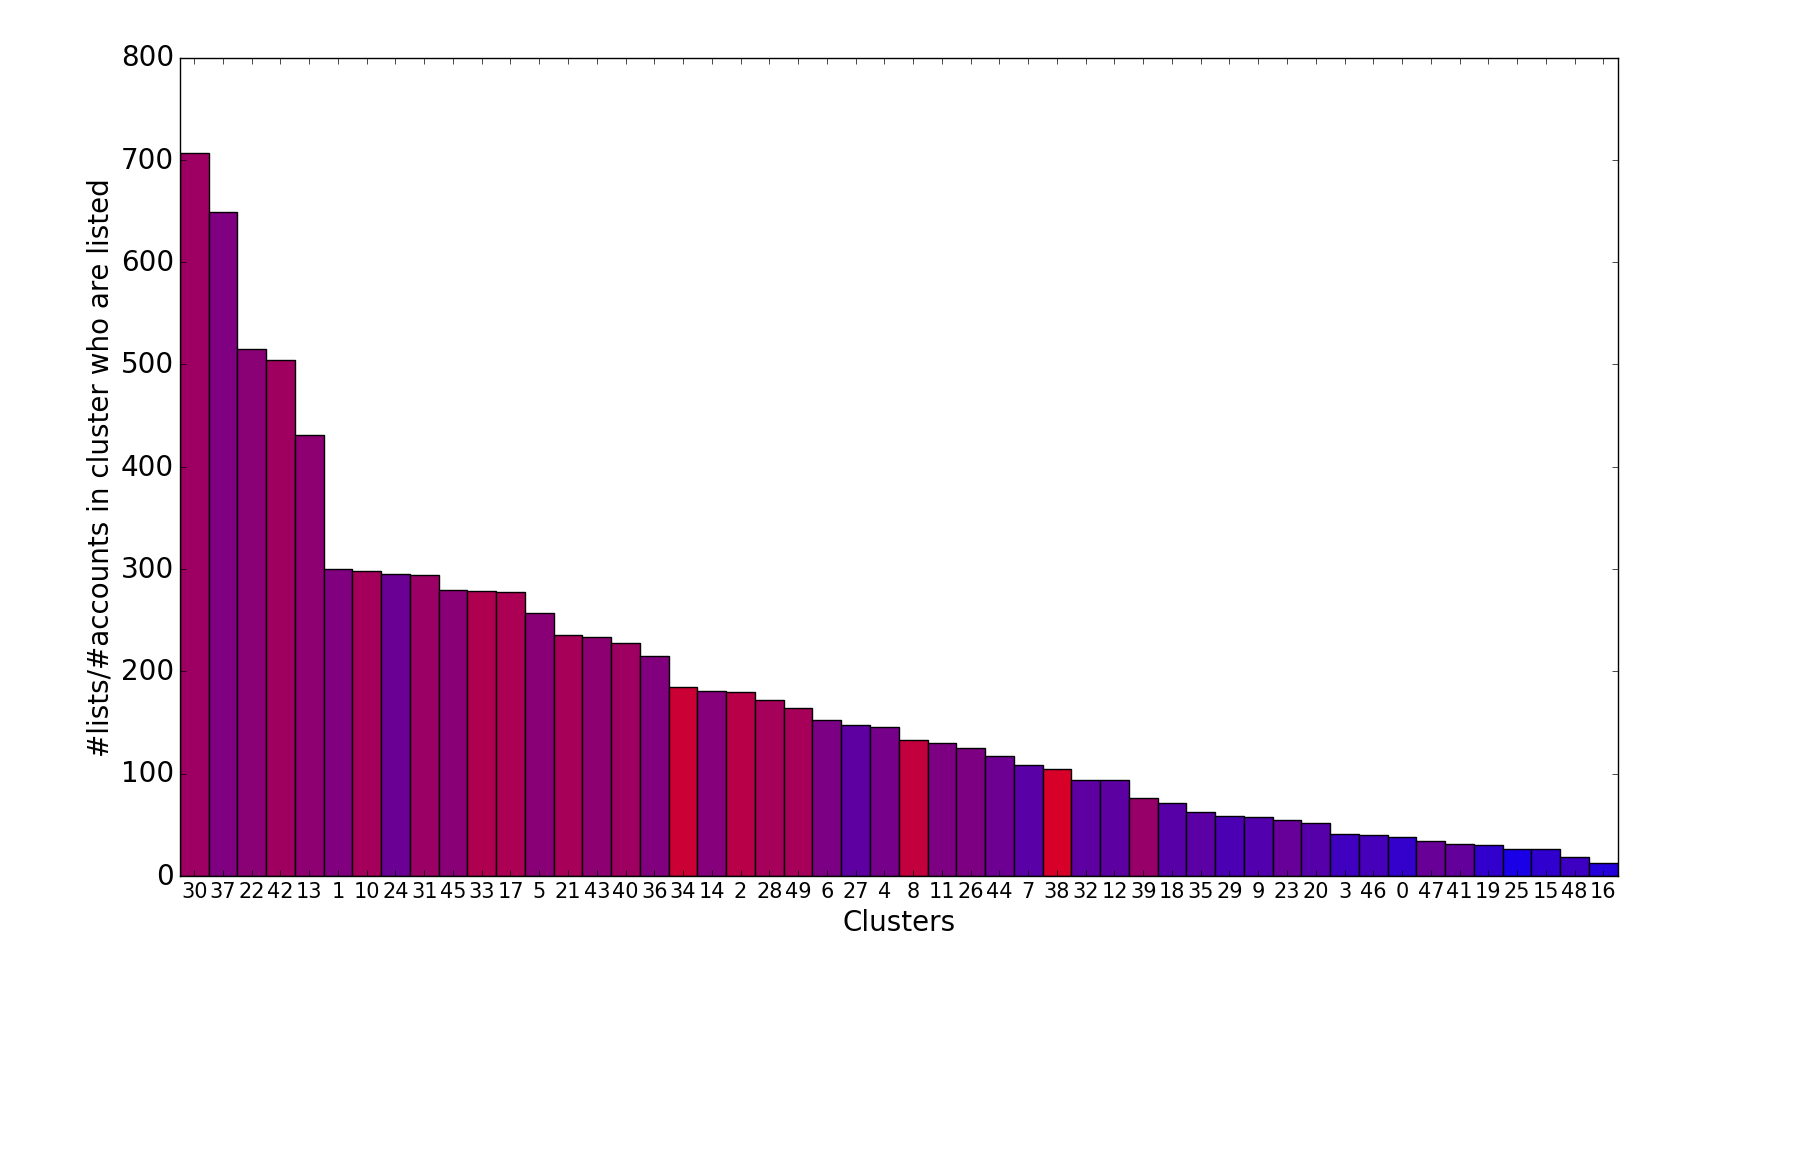
\includegraphics[width=0.5\textwidth]{imgs/listed2}
\end{figure}

\begin{figure}[h!]
	\caption{Presence In Lists Per Cluster}
	\centering
		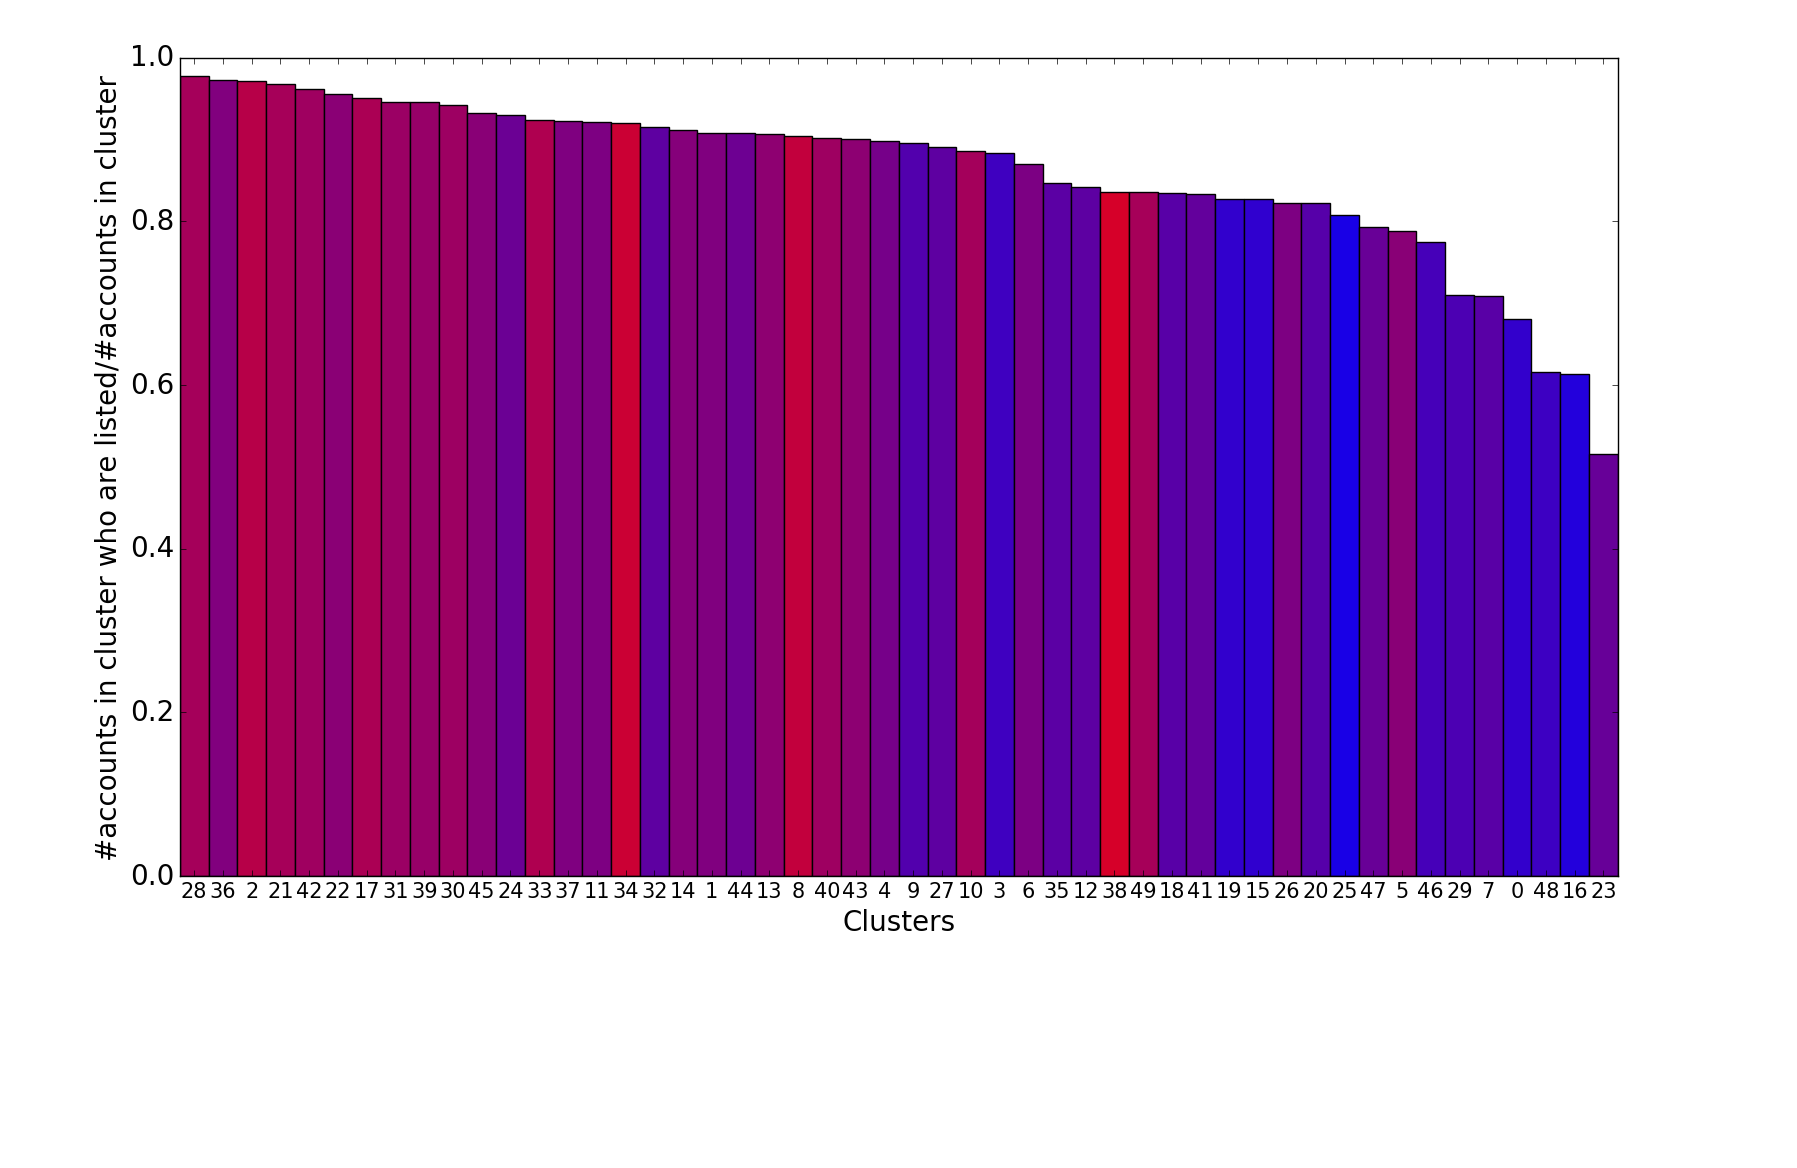
\includegraphics[width=0.5\textwidth]{imgs/listed3}
\end{figure}

%\balancecolumns % GM June 2007
% That's all folks!
\end{document}
